%% thesis.tex
%% 2013/05
%% by Sean Kenny
%% in Partial Fulfillment of the Requirements for the Degree of Master of Science

%--------------------------------------------------------------------------------------------
%------------------DOCUMENT STYLE ---------------------------------------------------------- 
%--------------------------------------------------------------------------------------------
\documentclass[12pt]{report}
\usepackage{abstract}
\usepackage[margin=1in]{geometry}
\usepackage{textcase}
\usepackage[utf8]{inputenc}
\usepackage{graphicx}
\usepackage{float}
\usepackage{listings}
\usepackage[titletoc]{appendix}
\usepackage[notindex,nottoc,notlot,notlof]{tocbibind}
\usepackage{tocloft}
\usepackage{helvet}
\usepackage{fullpage}
\usepackage{setspace}
\usepackage{titlesec}


\titleformat{\chapter}[hang]{\normalfont\large\center}{\MakeTextUppercase{\chaptertitlename}\ \thechapter:}{1em}{} 
% \titlespacing*{\chapter}{0pt}{0in}{1em}
\titleformat{\section}[hang]{\normalfont\large}{\thesection }{1em}{} 
\titleformat{\subsection}[hang]{\normalfont\large}{\thesubsection }{1em}{} 

\renewcommand{\abstractname}{\centering\normalfont\large\MakeTextUppercase{Abstract}}
\renewcommand{\contentsname}{\centering\normalfont\large\MakeTextUppercase{Table of Contents}}
\renewcommand{\cfttoctitlefont}{\hfill}
\renewcommand{\cftaftertoctitle}{\hfill}
\renewcommand{\listfigurename}{\centering\normalfont\large\MakeTextUppercase{List of Figures}}
\renewcommand{\cftloftitlefont}{\hfill}
\renewcommand{\cftafterloftitle}{\hfill}
\renewcommand{\cftchapfont}{}
\renewcommand{\cftchappagefont}{}
\renewcommand{\cftchappresnum}{CHAPTER }
\renewcommand{\cftchapaftersnum}{:}
\renewcommand{\cftchapnumwidth}{6.5em}
\renewcommand{\familydefault}{\sfdefault}
\renewcommand{\bibname}{\small\MakeTextUppercase{References}}

\doublespacing

\lstset{
         basicstyle=\footnotesize\ttfamily,
         numberstyle=\tiny,
         numbersep=5pt,
         tabsize=2,
         extendedchars=true,
         breaklines=true,
         showspaces=false,
         showtabs=false,
         showstringspaces=false   
 }

%--------- VARIABLES ---------- 
\newcommand{\rootPath}{../../}
\newcommand{\rootServerPath}{\rootPath server/}
\newcommand{\rootServerPhpPath}{\rootServerPath php/}
\newcommand{\rootClientPath}{\rootPath client/}
\newcommand{\rootClientJsPath}{\rootClientPath js/}

%--------- NEW COMMANDS ---------- 
%command for listing php files
\newcommand{\phplist}[1]{\lstinputlisting[language=PHP,basicstyle=\footnotesize\ttfamily,tabsize=2,numbers=left,frame=single,caption="#1"]{\rootServerPhpPath #1}}
 
%command for listing js files
\newcommand{\jslist}[1]{\lstinputlisting[language=Java,basicstyle=\footnotesize\ttfamily,tabsize=2,numbers=left,frame=single,caption="#1"]{\rootClientJsPath #1}}
\newcommand{\htmllist}[1]{\lstinputlisting[language=HTML,,basicstyle=\footnotesize\ttfamily,tabsize=2,numbers=left,frame=single,caption="#1"]{#1}}

%---------- NEW ENVIRONMENTS ----------
\newenvironment{dedication}
	{\vspace{6ex}\begin{quotation}\begin{center}\begin{em}}
	{\par\end{em}\end{center}\end{quotation}}


%---------- START THE DOCUMENT ----------
\begin{document}
\pagenumbering{roman}

%--------------------------------------------------------------------------------------------
%------------------ TITLE PAGE --------------------------------------------------------------- 
%--------------------------------------------------------------------------------------------
\newpage
\thispagestyle{empty}
\vspace*{\fill}
\begin{center}
	\large 
	\MakeTextUppercase{Implementation and Analysis of a} \\
	\MakeTextUppercase{Web Request Pipelining Framework} \\ 
	\MakeTextUppercase{By} \\
	\MakeTextUppercase{Sean Kenny} \\
	A Thesis Submitted to the School of Graduate Studies \\
	in Partial Fulfillment of the Requirements for the Degree of \\
	Master of Science \\
	\vspace{.5in}
	Southern Connecticut State University \\
	New Haven, Connecticut \\
	May 2013
\end{center}
\vspace*{\fill}

%--------------------------------------------------------------------------------------------
%------------------ SIGNATURE PAGE ---------------------------------------------------------- 
%--------------------------------------------------------------------------------------------
\newpage
\thispagestyle{plain}
\setcounter{page}{2}
\vspace*{0in}
\begin{center}
	\large 
	\MakeTextUppercase{Implementation and Analysis of a} \\
	\MakeTextUppercase{Web Request Pipelining Framework} \\ 
	\MakeTextUppercase{By} \\
	\MakeTextUppercase{Sean Kenny} \\
\end{center}
This thesis was prepared under the direction of the candidate's thesis advisor, Dr. Hrvoje Podnar, Department of Computer Science, and it has been approved by the members of the candidate's thesis committee. It was submitted to the School of Graduate Studies and was accepted in partial fulfillment of the requirements for the degree of Master of Science.

\begin{flushright}

\makebox[2in]{\hrulefill} \\
Hrvoje Podnar, Ph.D. \\
Thesis Advisor

\vspace{0.5in}

\makebox[2in]{\hrulefill} \\
Lisa Lancor, Ph.D. \\
Second Reader

\end{flushright}

\begin{flushleft}
\makebox[2in]{\hrulefill} \\
Imad Antonios, Ph.D. \\
Department Chairperson
\end{flushleft}


%--------------------------------------------------------------------------------------------
%------------------ ABSTRACT PAGE ----------------------------------------------------------- 
%--------------------------------------------------------------------------------------------
\begin{abstract}
\thispagestyle{plain}
\setcounter{page}{3}

\begin{flushleft}
\begin{tabular}{ll}
Author:  			& Sean Kenny 													\\
Title: 			& Implementation and Analysis of a Web Request Pipelining Framework	\\
Thesis Advisor: 	& Hrvoje Podnar, Ph.D.											\\
Institution: 		& Southern Connecticut State University								\\
Year: 			& 2012														\\
\end{tabular}
\end{flushleft}

\begin{flushleft}
This project intends to improve upon the current HTTP based web request and response system utilized by modern web browsers and servers today. This improvement will be made possible through the creation of a software HTTP web request pipelining library named OpenPipe. The OpenPipe library will attempt to increase the perceived speed of web content delivery through the optimization of communication sequences that occur during a standard HTTP web request cycle. The OpenPipe library will be provided as a PHP library for Apache based web servers, and a client side cross-browser JavaScript library. The existence of this library will allow for a greater level of transparency to web developers whom wish to provide advanced HTTP request pipelining  to their web sites and web application in a more plugable way, that can be extended to integrate with new and existing web based MVC frameworks. Once this library has been developed the final stage of this project will be to collect, analyze, and compare data for non-pipelined and pipelined web pages. The overall goal of this analysis will be to provide a clear picture of where the performance benefits occur when utilizing an HTTP request pipelining library that OpenPipe provides.
\end{flushleft}
\end{abstract}


%--------------------------------------------------------------------------------------------
%------------------ DEDICATION -------------------------------------------------------------- 
%--------------------------------------------------------------------------------------------
\begin{dedication}
\setcounter{page}{4}
\vspace*{\fill}
To my daughters, Paige and Jocelyn - for inspiration I will cherish always.
\linebreak\linebreak
To my wife, Kim - who’s selfless love, support, and encouragement has allowed me to fulfill new dreams and goals I never would have been able to imagine without her.
\vspace*{\fill}
\end{dedication}


%--------------------------------------------------------------------------------------------
%------------------ ACKNOWLEDGEMENT ------------------------------------------------------- 
%--------------------------------------------------------------------------------------------
\newpage
\thispagestyle{plain}
\setcounter{page}{5}
\vspace*{0in}
\begin{center}
\MakeTextUppercase{\large{Acknowledgements}} \\
\end{center}

I would like to thank Professor Hrvoje Podnar, who  in an exceptional way guided me through the thesis process and helped strengthen the research and results of this project.

I would also like to thank Professor Lisa Lancor, for her feedback and enthusiasm during all phases of this thesis's development.

\newpage


%--------------------------------------------------------------------------------------------
%------------------ TABLES ------------------------------------------------------------------- 
%--------------------------------------------------------------------------------------------
\tableofcontents
\listoffigures



%--------------------------------------------------------------------------------------------
%------------------INTRODUCTION ------------------------------------------------------------ 
%--------------------------------------------------------------------------------------------

\chapter{INTRODUCTION AND UNDERLYING TECHNOLOGIES}
\pagenumbering{arabic}

Modern web sites and web applications provide valuable information and services to an ever growing web audience. One of the most important requirements of web sites and web applications trying to deliver this important content is speed. Increased speed of a website can often determine an end user's perception of overall quality and value of a web-based service. Fast and responsive sites will be more likely to achieve higher monthly page views, adoption rates, and overall success.

The HTTP protocol is part of the application layer of the OSI model [see figure \ref{fig:osiModel}].  When an HTTP request is issued from a web browser for an initial HTML document, related elements such as images, JavaScript, and Cascading Style Sheet (CSS) are subsequently retrieved using additional HTTP requests. Therefore, the rendering of a single web page could involve many HTTP web requests. 

If speed is recognized as a critical factor for today's web then this current HTTP protocol used to deliver web content should be examined as the source of a possible bottleneck when trying to deliver performance. Web content has become increasingly more dynamic and interactive over the last ten years, and this current standard for web content delivery can be tailored for meeting the current pressures of the modern web. Since the introduction of HTTP, web developers have built an ever-growing repertoire of tips and tricks to squeeze the most out of the HTTP-based web. These methods include, but are not limited to the following \cite{highPerformanceWebsites}:

\begin{itemize}
	\item Use a content delivery network
	\item Add an Expires header (HTTP 1.1)
	\item Gzip components
	\item Put CSS at the top of the page
	\item Avoid CSS expressions
	\item Reduce DNS lookups
	\item Minify JS
	\item Avoid redirects
	\item Remove duplicate scripts
	\item Turn off ETags
	\item Make AJAX cacheable and small
\end{itemize}

Today's web sites and web applications employ many of these techniques to help deliver content to end-users in an efficient manner. HTTP Pipelining is another technique that could be employed alongside any of these methods to increase web performance.

 An HTTP pipeline is presented as a thin layer of application logic on top of HTTP which attempts to optimize the request cycle in a manner that allow pieces of a full web page to load and display independently.  This added layer is developed as a software library containing both server-side and client-side application code.

\begin{figure}[H]
\label{fig:osiModel}
\centering
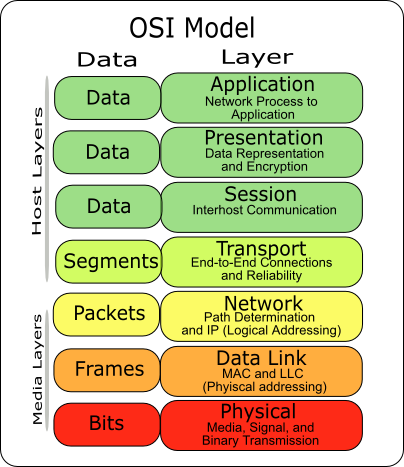
\includegraphics[width=90mm]{figures/images/osi_model.png}
\caption{Layers of the Open Systems Interconnection model (OSI model). OpenPipe resides in the application level of the OSI model.}
\end{figure}

The resulting library processes, requests, and delivers responses in an optimized manner taking into account current HTTP limitations that are inherent to the overhead created by the connect and request style of communication. The result of this response optimization through a pipeline is an increase in perceived speed that is accomplished by displaying fully functional content as quickly as possible – even before the entire document is completely processed by the web server.

HTTP pipelining is inspired from traditional pipelining technologies utilized by today’s modern CPU's, where an instruction's life cycle is broken into multiple stages. Instead of instructions, HTTP pipelining breaks the page generation process into several stages [see figure \ref{fig:HTTPRequestCycles}] which include \cite{facebookBigpipe}:

\begin{enumerate}
  \item Request parsing: web server parses and sanity checks the HTTP request. 
  \item Data fetching: web server fetches data from storage tier.
  \item Markup generation: web server generates HTML markup for the response. 
  \item Network transport: the response is transferred from web server to browser.
  \item CSS downloading: browser downloads CSS required by the page. 
  \item DOM tree construction and CSS styling: browser constructs DOM tree of the document, and then applies CSS rules on it.
  \item JavaScript downloading: browser downloads JavaScript resources referenced by the page.
  \item JavaScript execution: browser executes JavaScript code of the page.
\end{enumerate}

\begin{figure}[H]
\label{fig:HTTPRequestCycles}
\centering
\includegraphics[width=145mm]{figures/images/HTTP_request_cycles.jpg}
\caption{Comparison of a traditional HTTP web request with the operation of an HTTP web request Pipeline. A pipeline approach will deliver visible content sooner, as all parts of the  document are delivered in parallel.}
\end{figure}

Through the course of this paper we will review the implementation and design of an Opensource library called OpenPipe which implements a version of HTTP pipelining. This is accomplished through the development of both client and server side components that will be outlined in detail. Upon completion of the OpenPipe library testing and analysis was done to conclude how the differences in communication through HTTP pipelining really change the request and response times of a traditional client-server request model.


\section{PHP}
\begin{center} 

\includegraphics[width=30mm]{figures/images/php_logo.png}
\end{center}

The core server components of OpenPipe were all written with PHP 5.3. PHP is a general-purpose server-side scripting language originally designed for web development to produce dynamic web pages.

PHP can be deployed on most Web servers and as a standalone shell on almost every operating system and platform free of charge.  PHP is installed on more than 20 million Web sites and 1 million Web servers \cite{phpWiki}. These statistics make PHP a very good option to build and develop new web technologies and frameworks which will then be available to a large community of software developers.


\section{phpDocumentor}
\begin{center} 

\includegraphics[width=30mm]{figures/images/php_documentor_logo.png}
\end{center}

OpenPipe uses phpDocumentor to generate all of the available PHP class documentation. phpDocumentor is a tool with which it is possible to generate documentation from your PHP source code using a standardized set of source code commenting conventions. With this documentation you can provide developers with more information regarding the functionality embedded within your source code. phpDocumentor is heavily inspired by the JavaDoc tool available with the Java SDK. 


\section{CodeIgniter}
\begin{center}

\includegraphics[width=30mm]{figures/images/ci_logo.jpg}
\end{center}

The OpenPipe library that has currently been developed provides an adapter that interfaces with the CodeIgniter framework. Using this adapter it is fairly straight forward and simple to convert an existing CodeIgniter application to take advantage of OpenPipe HTTP request pipelining. CodeIgniter is a powerful PHP framework with a very small footprint, built for PHP coders who need a simple and elegant toolkit to create full-featured web applications. 


\section{Apache}
\begin{center} 

\includegraphics[width=30mm]{figures/images/apache_logo.png}
\end{center}

OpenPipe has been built and tested using the Apache HTTP server. OpenPipe is not limited to running on this architecture, and can theoretically be run on any web server that supplies integration with PHP.

Apache is a web server software notable for playing a key role in the initial growth of the World Wide Web. Apache is developed and maintained by an open community of developers under the Apache Software Foundation. Apache is available with many Linux distributions, and is freely available to download and compile. Prebuilt binary installers exist for all major operating systems.  

Since April 1996 Apache has been the most popular HTTP server software in use. As of March 2012 Apache was estimated to serve 57.46\% of all active websites and 65.24\% of the top servers across all domains \cite{webserverSurvey}.


\section{FireFox}
\begin{center} 

\includegraphics[width=30mm]{figures/images/firefox_logo.png}
\end{center}

All client side testing and analysis (manual and automated) of OpenPipe was performed using the FireFox web browser. FireFox supplies a very advanced toolset for profiling HTTP requests, viewing and editing HTML, and debugging JavaScript. FireFox is freely available to download and compile. Prebuilt binary installers exist for all major operating systems. 
 

\section{Selenium}
\begin{center}

\includegraphics[width=30mm]{figures/images/selenium_logo.png}
\end{center}

Selenium automates browsers by providing a common API that is provided in the form of a, 'WebDriver'. WebDrivers exist for every major browser including:

\begin{enumerate}
\item Firefox
\item Chrome
\item Safari
\item Internet Explorer
\item Android
\item iOS
\end{enumerate}

Selenium is primarily used for the automated testing of web applications, and is often used in conjunction with a unit testing framework.  Selenium is however not limited to this set of tasks and can be extremely useful for other tasks such as performance testing and analysis. OpenPipe utilized Selenium to help clarify the performance gains and penalties when using the framework under different usage scenarios and server load. Utilizing Selenium it became trivial to automate web page loading, and record large datasets of performance data.




%------------------------------------------------------------------------------------------------------
%--------------------ARCHITECURAL COMPONENTS--------------------------------------------------------- 
%------------------------------------------------------------------------------------------------------

\chapter{ARCHITECTURAL COMPONENTS}

\section{Client-server model}

OpenPipe delivers data from an HTTP server in a customized way that allows a corresponding client to interpret and render the data as soon as possible. Because of this OpenPipe is the combination of both server side and client side libraries working as complements to each. The server side components package and send data to the client, and the client side components unpack and utilize the received data [see figure \ref{fig:pipelinedRequestCycle}].

\begin{figure}[H]
\label{fig:pipelinedRequestCycle}
\centering
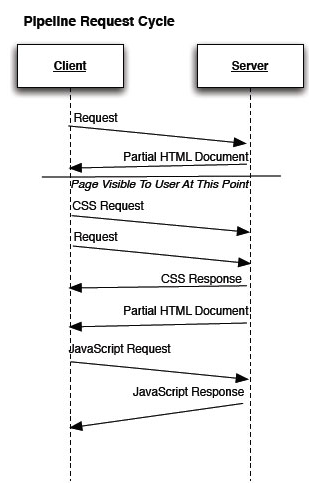
\includegraphics[width=65mm]{figures/images/pipeline_request_cycle.png}
\caption{A pipeline HTTP approach represented a traditional client-server communication process.}
\end{figure}




\section{Server components}

The server is composed of four main layers:

\begin{enumerate}
	\item \textbf{PHP} - The underlying scripting language. Run as a component of the web server.
	\item \textbf{OpenPipe\_Runner} - The main loop of an OpenPipe application. The runner orchestrates actions between the adapter being utilized, and the output that is generated.
		\begin{lstlisting}
//starting an openpipe runner
$openPipeRunner = new OpenPipe_Runner($openPipeAdapter, $openPipeOutput); $openPipeRunner->run(); //outputs openpipe content
		\end{lstlisting}

	\item \textbf{OpenPipe\_Adapter} - A plugable interface which retrieves and returns pipelets components from the underlying web framework. An adapter can be used to interface pre-existing PHP application frameworks with OpenPipe, or whole new OpenPipe-centric application frameworks.
		\begin{lstlisting}
//loading an openpipe adapter
$openPipeAdapter = OpenPipe_Adapter_Pvc_CodeIgniter(dirname(__FILE__));
		\end{lstlisting}	

	\item \textbf{Framework} - The framework being utilized with the OpenPipe adapter. The framework normally provides core web application components such as database libraries, request routing, session handling, and form validation. The CodeIgniter MVC system is an example of framework.
	
		\begin{figure}[H]
		\label{fig:frameworkStack}
		\centering
		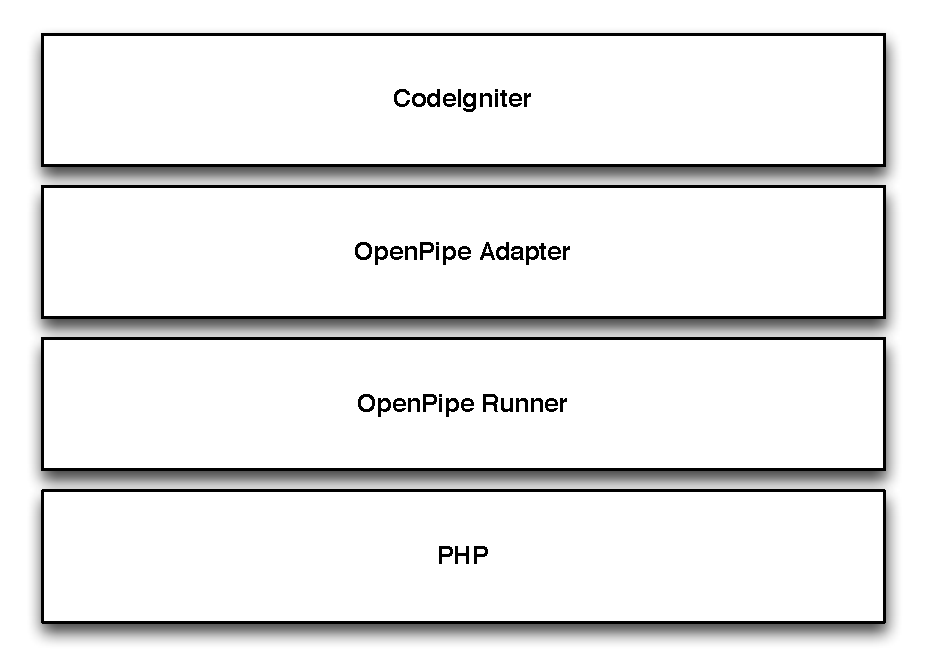
\includegraphics[width=\textwidth,keepaspectratio]{figures/images/framework_stack.pdf}
		\caption{Server side tecnology stack with OpenPipe components}
		\end{figure}

\end{enumerate}

\section{Client components}

The client is composed of three main layers:

\begin{enumerate}
	\item \textbf{JavaScript} - The host environment (web browser) and core JavaScript libraries.
	\item \textbf{Vendor Libraries} - OpenPipe makes use of two very popular, reliable, and lightweight cross-browser JavaScript frameworks.
		\begin{enumerate} 
			\item \textbf{Underscore.js} - A utility-belt library for JavaScript that provides functional programming support.
			\item \textbf{jQuery} - Provides simple and elegant client side scripting and manipulation of HTML DOM.
		\end{enumerate}
	\item \textbf{OpenPipe} - A client side library which is responsible for receiving events from an OpenPipe based server. These events are processed and associated data for these events is loaded into the HTML DOM as HTML, CSS, and JavaScript.
		
		\begin{figure}[H]
		\label{fig:clientFrameworkStack}
		\centering
		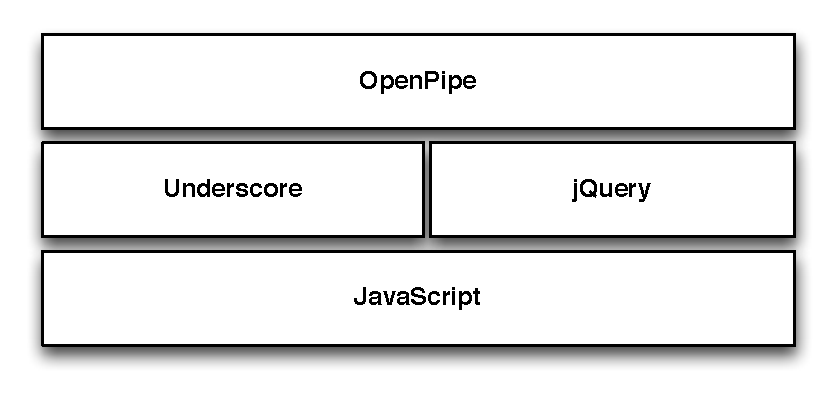
\includegraphics[width=\textwidth,keepaspectratio]{figures/images/client_stack.pdf}
		\caption{Client side tecnology stack with OpenPipe components}
		\end{figure}

\end{enumerate}




%------------------------------------------------------------------------------------------------------
%--------------------PIPELETS--------------------------------------------------------------------------
%------------------------------------------------------------------------------------------------------


\chapter{PIPELETS}

Every OpenPipe HTTP request cycle is composed of pipelets. A pipelets represents an atomic composition of HTML, CSS, and JavaScript [see figure \ref{fig:samplePipelet}] . A web page request can be composed of one to many pipelets.

\begin{figure}[H]
\label{fig:samplePipelet}
\begin{lstlisting}
<!-- a simple pipelet containing css, javascript, and html -->
<div pipelet-id="pipelet-1" ></div>
	<link rel="stylesheet" type="text/css" href="css/pipelet-1.css" />
	<script type="text/javascript" src="js/pipelet-1.js" ></script>
	<h1>Hello world!</h1>
</div>
\end{lstlisting}
\caption{Sample pipelet containing HTML, CSS, and JavaScript}
\end{figure}


\section{The Root Pipelet}
Every pipelined HTTP request contains at least one initial pipelet. This initial pipelet is known as the root pipelet, and is the source for extraction and retrieval for all other pipelets. The root pipelet is special because it defines the overall layout of the page, from which all pipelets will be loaded and placed into [see figure \ref{fig:sampleRootPipelet} and \ref{fig:rootPipeletLayout}]. 
	
The root pipelet contains the root \textless html /\textgreater\ element and its immediate children - \textless head /\textgreater\ and \textless body /\textgreater\	. Since the root pipelet defines the head section it is capable of setting extra page meta information through specialized head tags, and linking or including CSS and JavaScript shared between pipelets.

\begin{figure}[H]
\label{fig:sampleRootPipelet}
\begin{lstlisting}
<html>
<head>
<title>Root Pipelet!</title>
<link rel="stylesheet" type="text/css" href="css/global.css" />
<script type="text/javascript" src="js/app.js" ></script>
</head>
<body>
<h1>Hello World!</h1>
<div pipelet-id="pipelet-1"></div>
<div pipelet-id="pipelet-2"></div>
</body>
</html>
\end{lstlisting}
\caption{Root piplet HTML}
\end{figure}


\begin{figure}[H]
\label{fig:rootPipeletLayout}
\centering
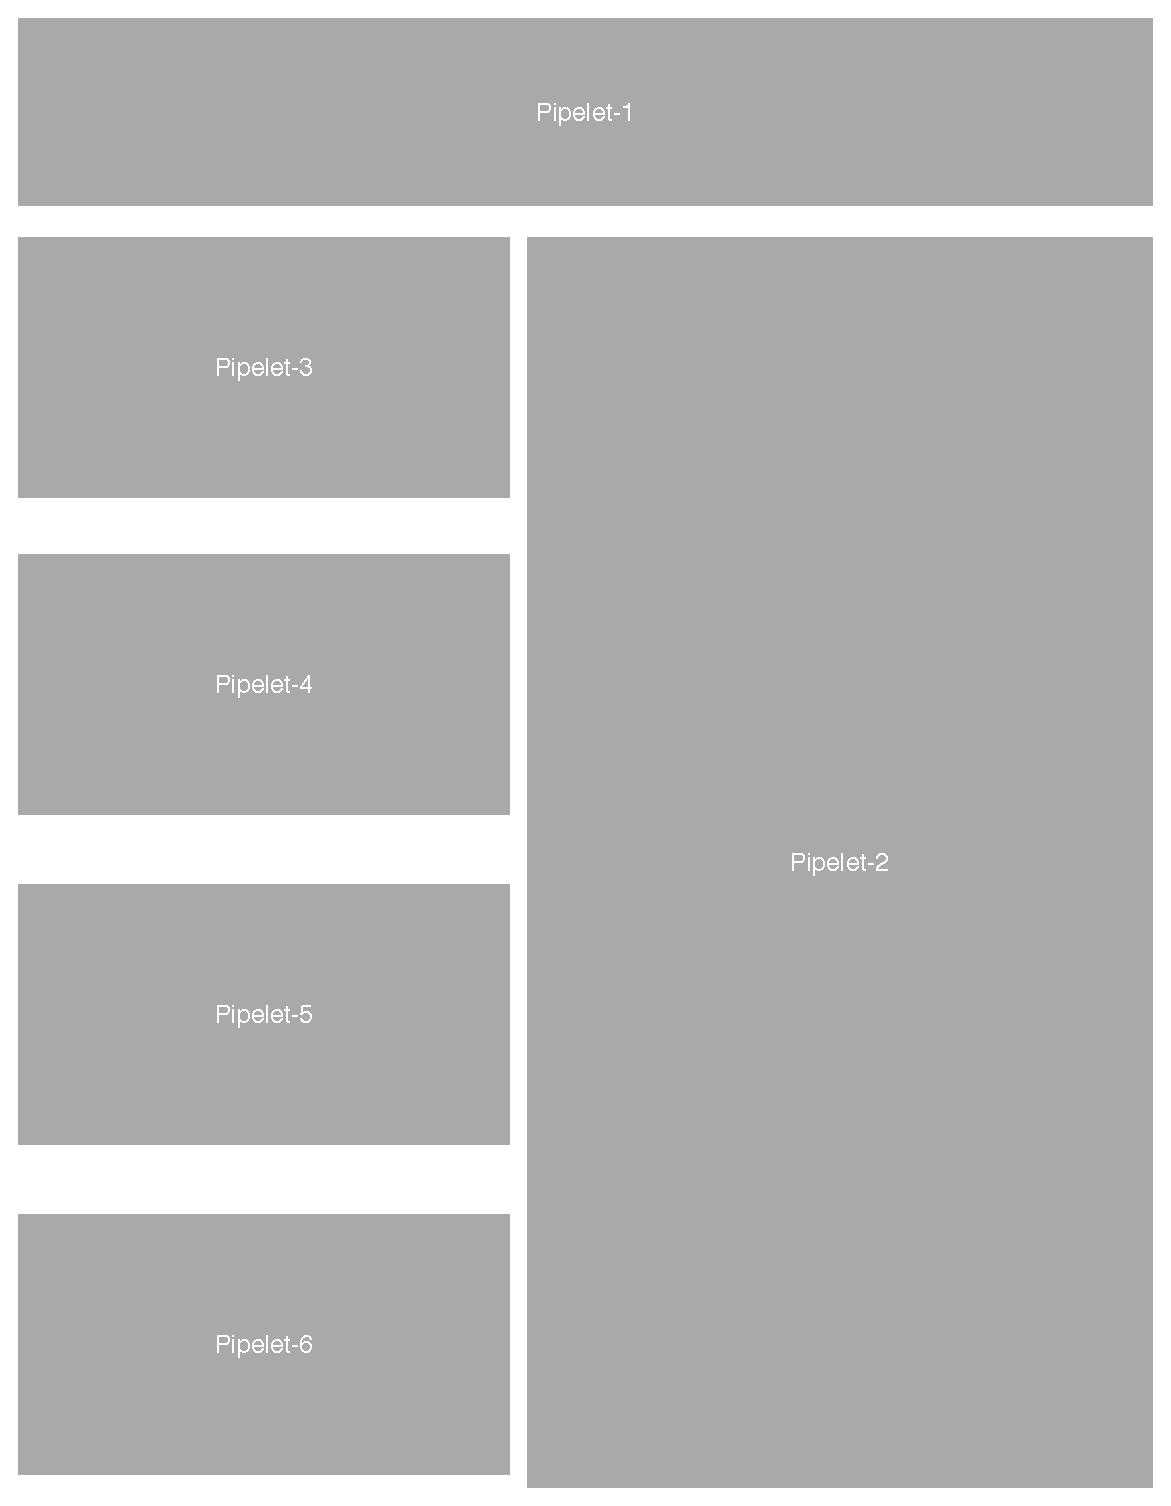
\includegraphics[width=\textwidth,keepaspectratio]{figures/images/root_pipelet.pdf}
\caption{Root pipelet layout}
\end{figure}

	
\section{Nested Pipelets}
Pipelets can be nested within other pipelets. This provides a mechanism to display content that contains n-levels of content depth, and allows for a great deal of flexibility when dealing with nested retrieval and display of data within a web page. Using nested pipelets the page being rendered can start to be divided into subcomponents, and those subcomponents can have more subcomponents of their own. 

Figure \ref{fig:nestedPipelets} illustrates a nested pipelet page of depth 3. Each set of pipelets is loaded using a breadth first loading algorithm. So all the pipelets at depth n will be loaded and rendered before the system continues to load pipelets at depth n+1. Its also important to note that loading of JavaScript for all pipelets will be deferred until all pipelet content (HTML and CSS) has been loaded for the given depth.

\begin{figure}[H]
\label{fig:nestedPipelets}
\centering
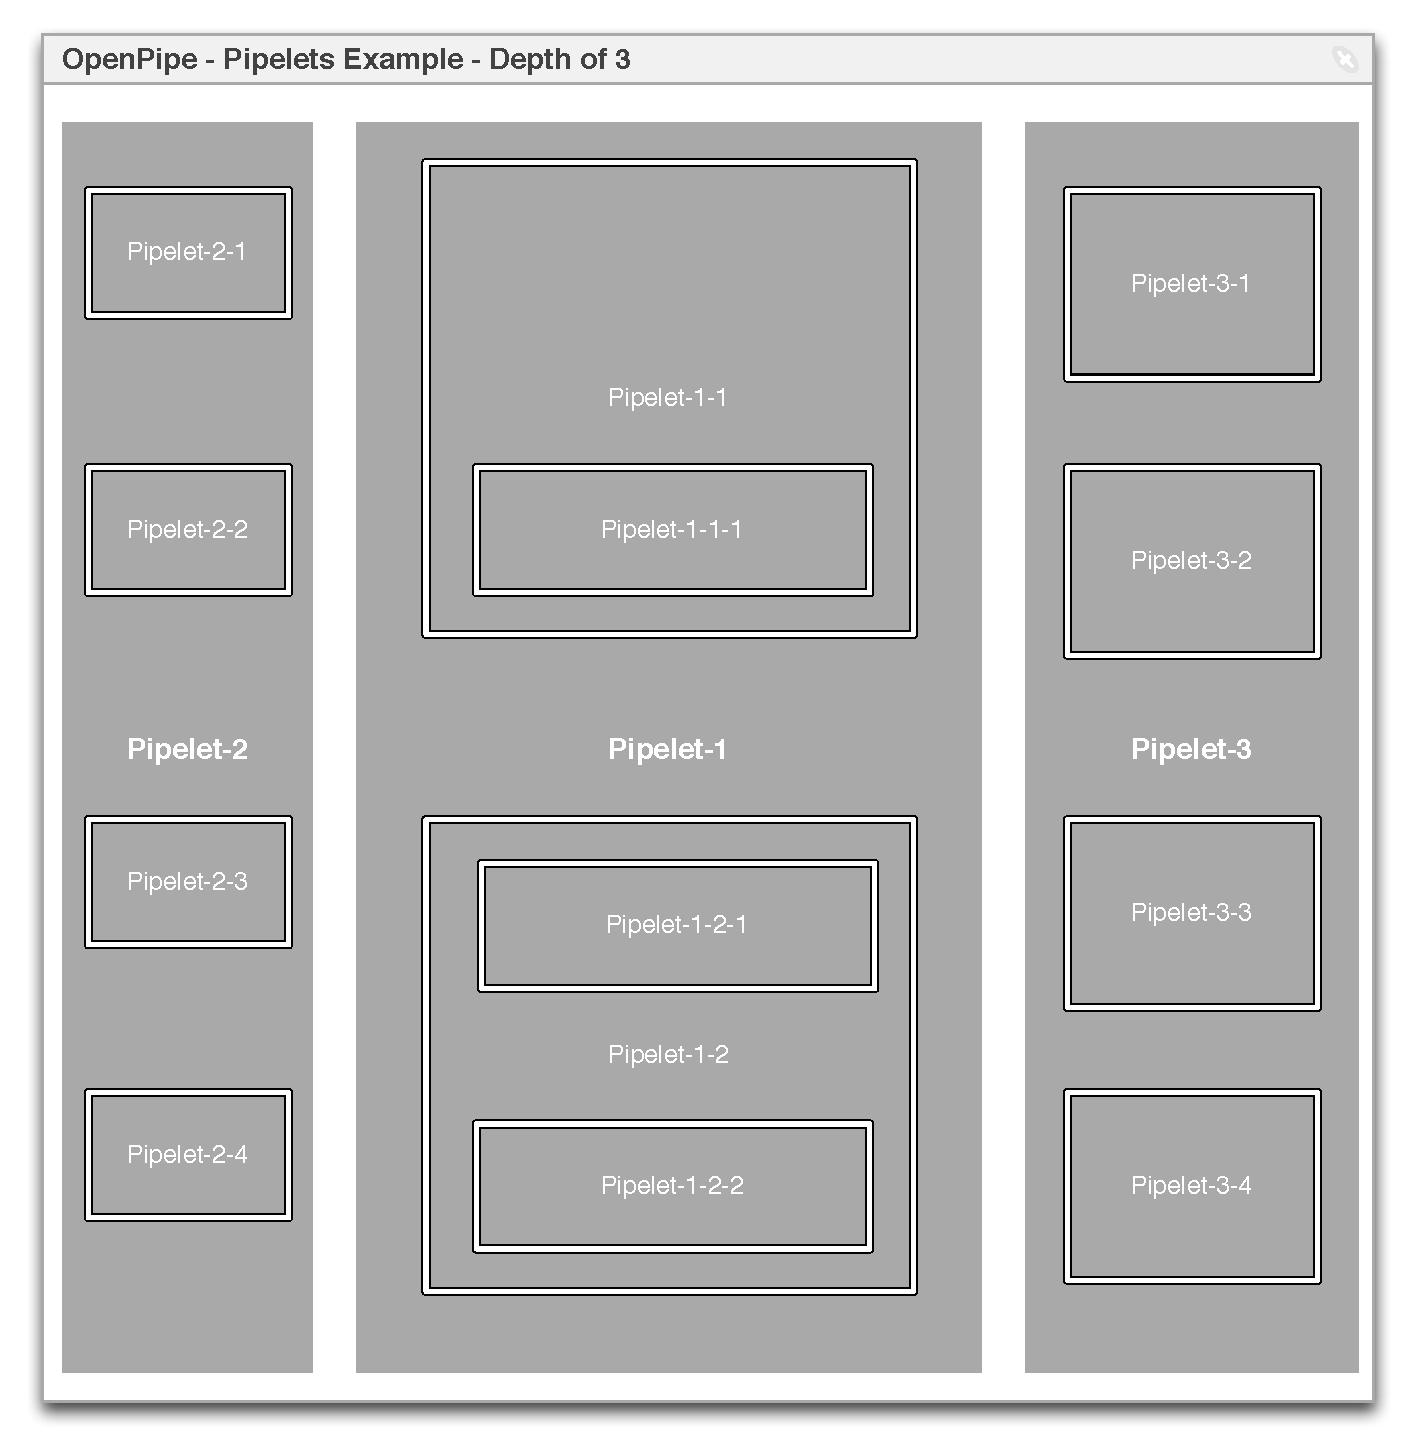
\includegraphics[width=\textwidth,keepaspectratio]{figures/images/nested_pipelets.pdf}
\caption{Nested Pipelets with a depth of 3}
\end{figure}

\section{Pipelet Priority}

Pipelets that are part of the same depth can prioritized explicitly using the pipelet-priority OpenPipe HTML attribute [see figure \ref{fig:pipeletPriority}]. By default all pipelets are loaded in ascending alphanumeric order of the pipelet\_id OpenPipe HTML attribute. The addition of an explicit pipelet\_priority tag allows for a greater degree of control when loading pipelet components and, most importantly allows for the developer to choose which pieces of the page should be loaded and transmitted first.

\begin{figure}[H]
\label{fig:pipeletPriority}
\begin{lstlisting}
<!-- a root pipelet -->
<html>
<head>
<title>Root Pipelet!</title>
	<link rel="stylesheet" type="text/css" href="css/global.css" />
	<script type="text/javascript" src="js/app.js" ></script>
</head>
<body>
	<h1>Hello World!</h1>
	<div pipelet-id="pipelet-1"></div>
	<div pipelet-id="pipelet-2" pipelet-priority="1" ></div>
</body>
</html>
\end{lstlisting}
\caption{Sample pipelet containing HTML, CSS, and JavaScript}
\end{figure}




%------------------------------------------------------------------------------------------------------
%--------------------CLASS INTERFACES------------------------------------------------------------------
%------------------------------------------------------------------------------------------------------

\chapter{CLASS INTERFACES}

OpenPipe defines core interfaces for pluggable components of the system. Through utilizing provided interfaces developers can contour and extend the library to meet new and existing needs. 

\section{Output}

\begin{figure}[H]
\label{fig:generalizationOutput}
\centering
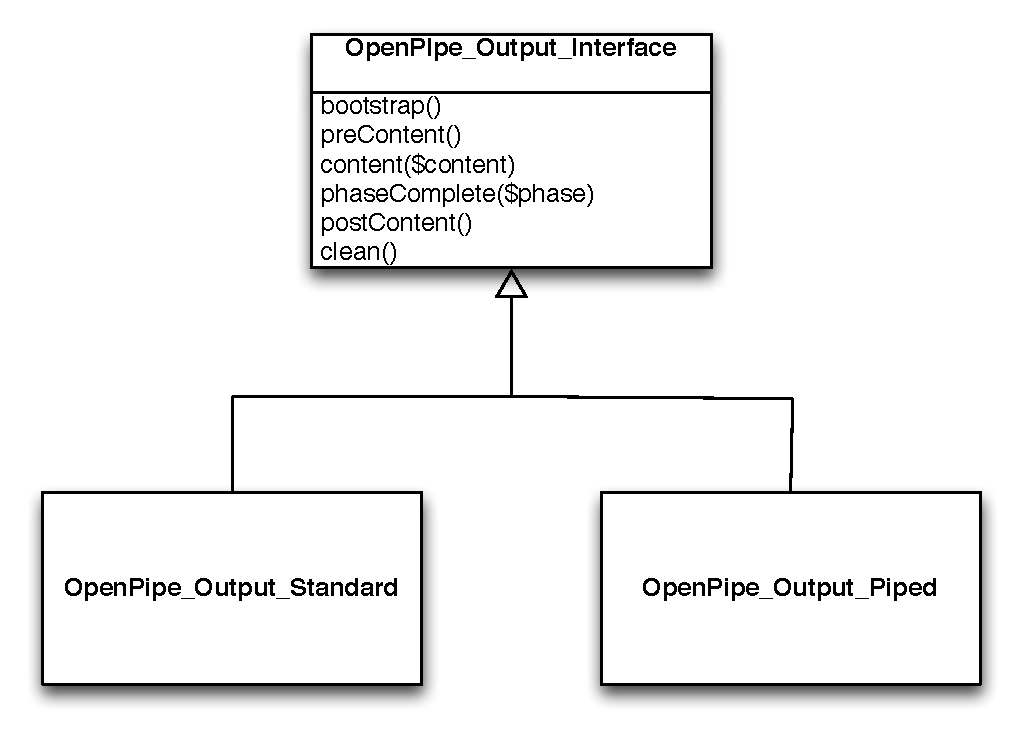
\includegraphics[width=\textwidth,keepaspectratio]{figures/images/generalization_output.pdf}
\caption{A generalization of the OpenPipe output object}
\end{figure}

The output interface [see figure \ref{fig:generalizationOutput}] defines how to conform to a set of output principles that allow for desired output functionality depending on the needs and capability of the client accessing an OpenPipe based web page.  The output interface defines the following methods:

\begin{enumerate}
	\item \textbf{bootstrap} - Allows implementor to setup and output any data before the content phase begins.
	\item \textbf{preContent} - Called immediately before any content is to be outputted through the associated content() method. 
	\item \textbf{output} - Called when content is ready for output - This content is already generated HTML string.
	\item \textbf{phaseComplete} - Called when an output phase is complete. A phase represents a layer of data (each layer of data can contain n number of deeper layers).
	\item \textbf{postContent} - Called immediately after all data has been sent for output.
	\item \textbf{clean} - Allows implementor to do any final cleanup and output. This is the last step in the output process.
\end{enumerate}

Out of the box the core OpenPipe library provides two output interface implementations:

\begin{enumerate}
	\item \textbf{OpenPipe\_Output\_Piped} - Implementation of an OpenPipe output interface that sends data by way of an HTTP pipeline. This is done by loading the openpipe.js client library and associated libraries. The output handler handles extracting pipelet HTML data, and transmitting it as packed JSON object, which will be unpacked by the client openpipe.js library.
	\item \textbf{OpenPipe\_Output\_Standard} - Implementation of an OpenPipe output interface that sends data as a standard HTML document. Content pieces are used to construct a complete HTML document, placing CSS and JavaScript in proper placement, and inject each content piece within a pipelet place holder on the server side. It's important to note that no javascript is required to complete output on the client web browser while using this output implementation.
\end{enumerate}

This illustrates the power of decoupling the output system into an interface which is chosen at runtime based on the needs and capabilities of a given client receiving the output information. Through the use of the same output interface the OpenPipe runner can transparently interface with JavaScript capable devices and non JavaScript capable devices such as web crawlers and bots without needing to alter any information retrieved from a corresponding framework interface.


\section{Framework Adapter}

\begin{figure}[H]
\label{fig:generalizationAdapter}
\centering
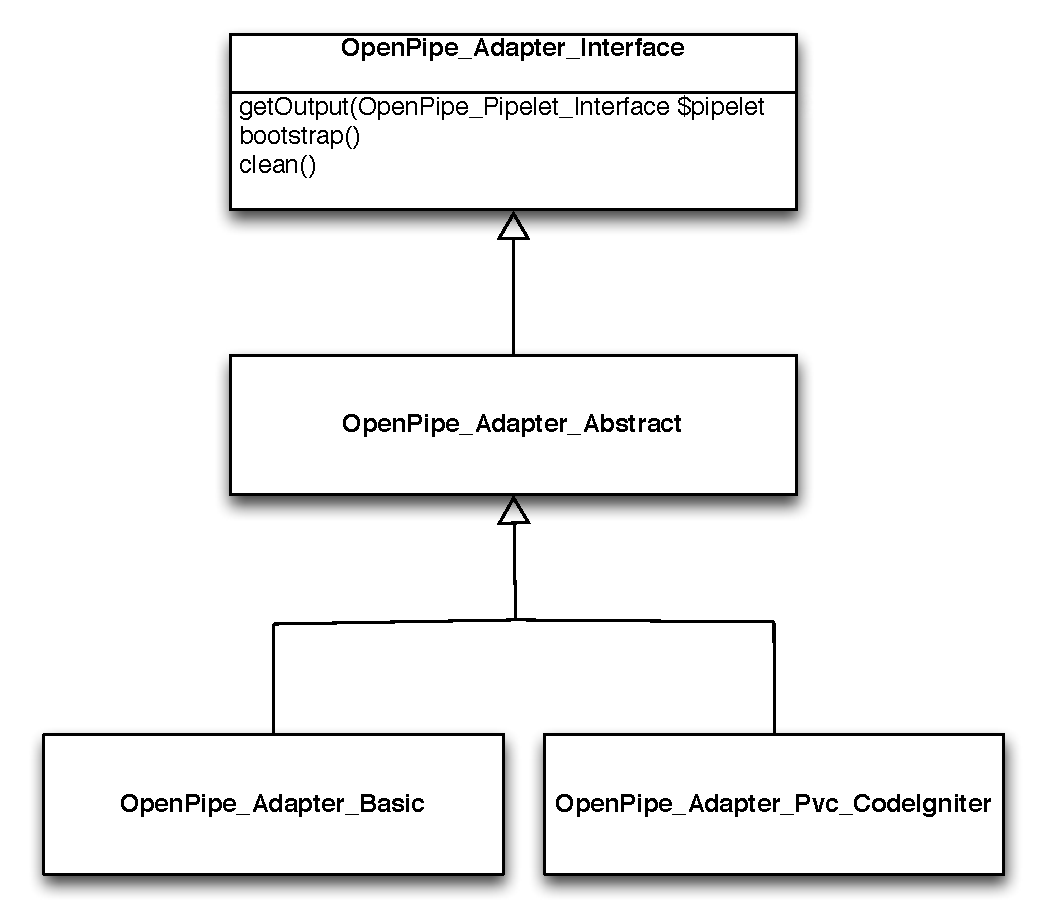
\includegraphics[width=\textwidth,keepaspectratio]{figures/images/generalization_adapters.pdf}
\caption{A generalization of the OpenPipe adapter object}
\end{figure}

A framework's adapter [see figure \ref{fig:generalizationAdapter}]  is a crucial component of the OpenPipe library that converts web requests into underlying framework routing requests. These routing requests result in output. The output for each request is returned by the framework adapter to the OpenPipe output interpreter where it is parsed for more web requests that need to retrieved by the framework adapter. This process continues until all output is retrieved.





%------------------------------------------------------------------------------------------------------
%--------------------DESIGN PATTERNS-------------------------------------------------------------------
%------------------------------------------------------------------------------------------------------
\chapter{DESIGN PATTERNS}

The OpenPipe library utilizes design patterns where appropriate to make the available components easier to comprehend from a conceptial level, and also easier to extend for future use. The patterns explained below were chosen to provide maximum flexibility to the underlying system when integrating with existing PHP web application systems and frameworks.

\section{Strategy Pattern}

OpenPipe uses the strategy design pattern to define families of objects that can be utilized by the OpenPipe\_Runner class at runtime [see figure \ref{fig:strategyRunner}]. This helps effectively decouple the OpenPipe\_Runner from rendering and output concerns. These two concerns can vary depending on:

\begin{enumerate}
	\item The type of HTTP client accessing the web page (web browser, bot, crawler).
	\item The type of framework that OpenPipe is using to access and render web page information (CodeIgniter, Zend Framework, CakePHP).
\end{enumerate}

\begin{figure}[H]
\label{fig:strategyRunner}
\centering
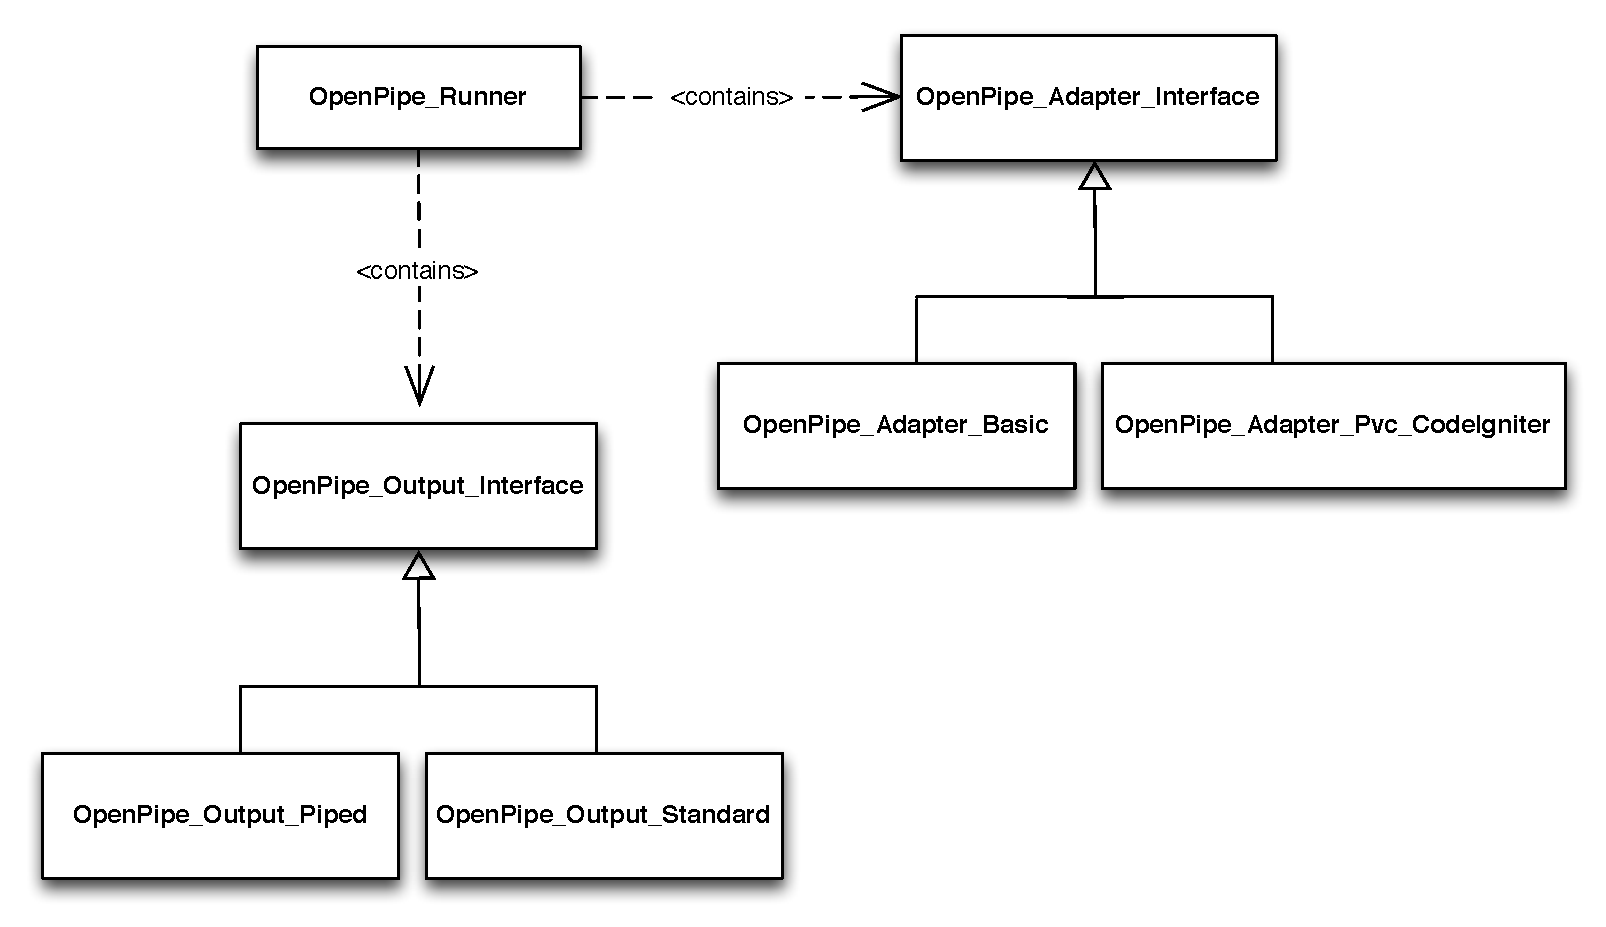
\includegraphics[width=\textwidth,keepaspectratio]{figures/images/strategy_runner.pdf}
\caption{The strategy pattern utilzed by OpenPipe for the main OpenPipe runner object}
\end{figure}

Another benefit of this design pattern implementation is that new adapters and output classes can be developed and utilized in the future. Once created they only need to be passed as parameters to the OpenPiper\_Runner class when it is instantiated [see figure \ref{fig:strategyRunnerCode}].

\begin{figure}[H]
\label{fig:strategyRunnerCode}
\begin{lstlisting}
//starting an openpipe runner
$openPipeRunner = new OpenPipe_Runner($openPipeAdapter, $openPipeOutput); 
$openPipeRunner->run(); //outputs openpipe content
\end{lstlisting}
\caption{Instantiation and running of an OpenPipe\_Runner object}
\end{figure}


\section{Factory Pattern}

OpenPipe utilizes the factory design pattern to construct pipelets from output received from a framework adapter [see figure \ref{fig:factoryPattern}]. The factory receives raw HTML data and current phase information. The factory then continues to parse embedded pipelet information from the HTML and return an array of Pipelets that conform to the OpenPipe\_Pipelet\_Interface 

\begin{figure}[H]
\label{fig:factoryPattern}
\centering
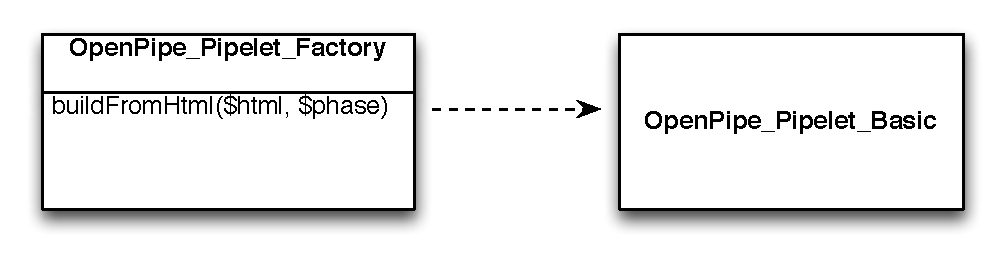
\includegraphics[width=\textwidth,keepaspectratio]{figures/images/factory_pipelets.pdf}
\caption{The factory pattern utilized by OpenPipe}
\end{figure}




%------------------------------------------------------------------------------------------------------
%--------------------SEQUENCE DIAGRAMS ----------------------------------------------------------------------
%------------------------------------------------------------------------------------------------------
\chapter{SEQUENCE DIAGRAMS}

\section{Server}

Every open pipe request cycle is handle by a core class named OpenPipe\_Runner. The runner is responsible for orchestration communication with a class that implements the OpenPipe\_Adapter interface. This communication results in:

\begin{enumerate}
\item Notification of bootstrapping and cleanup stages in the request cycle.
\item Retrieval of the root pipelet content (layout).
\item Retrieval of nested pipelets within the root pipelet.
\end{enumerate}

Once the OpenPipe\_Runner class has received information from the OpenPipe\_Adapter its passes any renderable content to a class that implements the OpenPipe\_Output interface. The OpenPipe\_Output class handles sending data to the client, and removes any special concerns for how this data is transmitted away from the OpenPipe\_Runner.

The OpenPipe\_Runner is also responsible for calling upon a Pipelet\_Factory to build pipelets from content gathered from the Pipelet\_Adapter. The Pipelet\_Factory returns an array of pipelets which contain information that can be sent to the OpenPipe\_Adapter to gather the pipelet HTML and data, and then passed to the OpenPipe\_Output class for rendering. The factory process is the main loop in the OpenPipe\_Runner application.

All components of this process are pluggable and determined at runtime. The OpenPipe\_Runner class depends only on the individual interfaced defined in the OpenPipe library, and utilizes specific design patterns such as the strategy and factory patterns to decouple it directly from any class instantiation.

The sequence diagram for a complete OpenPipe request is outline in figure \ref{fig:openPipeRunnerSequenceDiagram}

\begin{figure}[H]
\label{fig:openPipeRunnerSequenceDiagram}
\centering
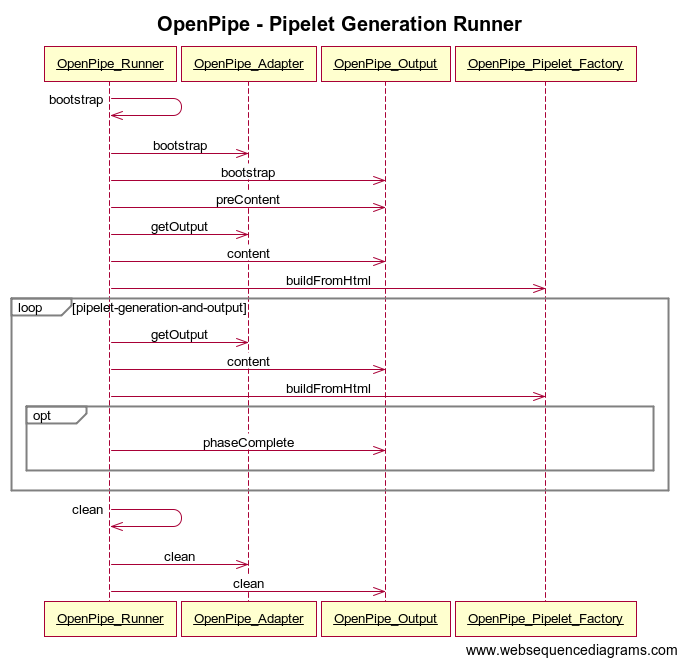
\includegraphics[width=\textwidth,keepaspectratio]{figures/images/openpipe_runner.png}
\caption{OpenPipe Runner sequence diagram}
\end{figure}

\section{Client}

Once a request is handled and output is sent through an OpenPipe\_Output class, this output must be interpreted and acted upon by a the OpenPipe client library.  The client library is built entirely of JavaScript and contains the following API calls:

\begin{enumerate}
\item \textbf{init} - this is called during the main page layout initialization stage. It handles setting up the layout and initializing the client library so it can load additional segments.
\item \textbf{loadSegment} - this is the main method call, which handles loading pipelet data from the server and rendering it within a web browser. It accepts segment data, which are essentially predefined JSON objects.
\item \textbf{registerPhase} - called when a segment is loaded. If the segment part of  a new phase then the phase is recorded as starting and any script received will be queued until this phases content (HTML and CSS) has been loaded and rendered.
\item \textbf{loadCss} - loads a given array of CSS elements (\textless link /\textgreater\ and \textless style /\textgreater\ tags). The CSS information is inserted directly into the \textless head /\textgreater\ section of the HTML document].
\item \textbf{loadHtml} - load a given HTML document into the layout’s pipelet placeholder. The placeholder to insert content to is determined using the segments corresponding id.
\item \textbf{pushScripts} - pushes a segment's set of script tags (both inline and external) onto a stack for later retrieval. JavaScript is loaded at the end of each loading phase. This allows for content represented as HTML and CSS to be loaded and viewable first before any possibly long JavaScript execution takes place.
\item \textbf{phaseComplete} - marks a phase as complete. When a phase is marked complete all JavaScript queued from segments loaded during the same phase will be appended to the \textless head /\textgreater\ section of the HTML document and executed in the order received.
\end{enumerate}

The sequence diagram for a complete OpenPipe client processing cycle is outlined in figure \ref{fig:openPipeClientOutputSequenceDiagram}

\begin{figure}[H]
\label{fig:openPipeClientOutputSequenceDiagram}
\centering
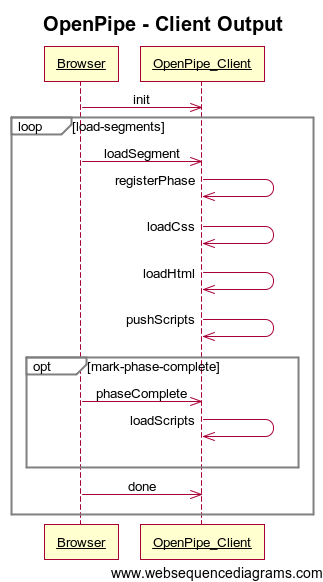
\includegraphics[width=80mm]{figures/images/openpipe_clientoutput.png}
\caption{OpenPipe output sequence diagram}
\end{figure}

\begin{figure}[H]
\label{fig:openPipeClientPipeletLoadCalls}
\begin{lstlisting}
<html>
<head>
	<title>OpenPipe Sample Page</title>
	<script type="text/javascript" src="js/libs/jquery.js"></script>
	<script type="text/javascript" src="js/libs/underscore.js"></script>
	<script type="text/javascript" src="js/openpipe.js"></script>
</head>
<body>
	<div id="container" ><!-- root layout data. --></div>
	<!-- followed by openpipe client request calls -->
	<script type="text/javascript">
	op.load({...});
	</script>
	<script type="text/javascript">
	op.load({'id':'pipelet1', 'html': '...', 'css': [], 'scripts': []});
	</script>
	<script type="text/javascript">
	op.load({'id':'pipelet2', 'html': '...', 'css': [], 'scripts': []});
	</script>
	<script type="text/javascript">
	op.load({'id':'pipelet3', 'html': '...', 'css': [], 'scripts': []});
	</script>
	<script type="text/javascript">
	op.phaseComplete(1); op.done();
	</script>
</body>
</html>
\end{lstlisting}
\caption{OpenPipe client side pipelet load calls}
\end{figure}




%------------------------------------------------------------------------------------------------------
%-------------------- Other Library Components -----------------------------------------------------------
%------------------------------------------------------------------------------------------------------
\chapter{OTHER LIBRARY COMPONENTS}

\section{Transmitted Data}

Pipelet data is transmitted as JSON to the client. Each individual pipelet transmitted as JSON is referred to as a segment in the OpenPipe.js client library. A segment contains the following data elements [see figure \ref{fig:clientSegmentDataObject}]:

\begin{enumerate}
\item \textbf{ID} - the id of the pipelet the information in the segment pertains to. 
\item \textbf{CSS} - an array of inline and external css HTML tags. This information is extracted from the server output and organized before transmission to the client as a segment.
\item \textbf{Scripts} - an array of inline and external script HTML tags. This information is extracted from the server output and organized before transmission to the client as a segment.
\item \textbf{HTML} - raw HTML data that is left after css and script data extraction.
\end{enumerate}

\begin{figure}[H]
\label{fig:clientSegmentDataObject}
\centering
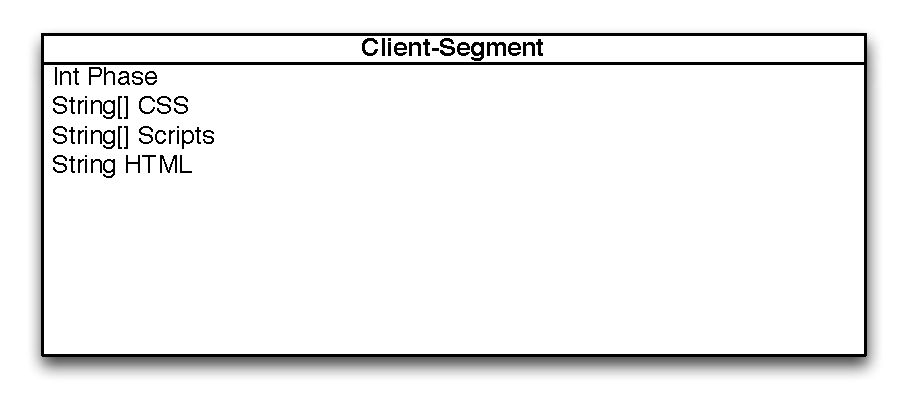
\includegraphics[width=\textwidth,keepaspectratio]{figures/images/client_segment_data_object.pdf}
\caption{The client segment data object}
\end{figure}

\section{PHP Output Buffering}
PHP has built in functionality which prevents output data from being transmitted
to a client connection until a certain amount of data has been placed into an output buffer. This however is counter productive to the operation of OpenPipe since each pipelet needs to be transferred immediately after is ready for output. This allows for the illusion of page rendering speed. If the buffer was left in place PHP would not output the data in a continuous stream and the experience would be similar to non HTTP Pipelined pages. 

To get around this issue OpenPipe utilizes a custom output utility class which provides an output function named echoNow [see figure \ref{fig:echoNowCode}]. echoNow performs similarly to the standard echo function in PHP, but it is output buffer aware. Every time the echoNow function is called it queries the current PHP output buffer size and pads the output string with as much data that is needed so that the buffer will be full and the output data will be sent immediately. Utilizing this function classes within the OpenPipe library to not need to individually carry the concern of output buffering and how to circumvent it.

\begin{figure}[H]
\label{fig:echoNowCode}
\begin{lstlisting}
/**
* Highly reusable output method which echos data NOW - by NOW we mean in an intelligent way that takes into account output buffering in PHP
* as well as browser based deferred display of data (until data is of x bytes) - Using this utility method one should not have to worry about how 
* to immediately send data to an end client browser NOW
* @param string $output the data to output NOW!
* @param int|null $outputBufferSize the output buffer currently in use -if a string is not of an output buffer length it will be padded to meet the minimum buffer size - If not provided this value will be looked up from the PHP ini configuration value 
* @param string $paddingCharacter the character to pad output with if the buffer is larger than the data to output
*/
public static function echoNow($output, $outputBufferSize=null, $paddingCharacter = ' '){

//if the output buffer is null, then attempt to get it from php ini
if($outputBufferSize === null){
	$outputBufferSize = @ini_get('output_buffering');
	if($outputBufferSize == 'Off') $outputBufferSize = 0;
}
		
//now that we know the buffer check to see how much we need to pad the string that is to be outputted
$bufferSpace = $outputBufferSize - strlen($output);
if($bufferSpace > 0){
	$output = $output.str_repeat($paddingCharacter, $bufferSpace);
}

//echo the string (with possible padding), then flush!
echo $output;
flush();
}
\end{lstlisting}
\caption{PHP function that helps bypass PHP output buffering that blocks the HTTP pipelining of data to the client browser}
\end{figure}


\section{Dynamic JavaScript DOM Insertion}

Inserting JavaScript into an existing DOM document needs to be done in a slightly different way than just appending the raw JavaScript data to the current HTML document being loaded. To do this in a reliable and cross browser way the boiler plate DOM function, 'createElement', is used to create a new script tag. Once the script tag is created the type and source code attributes are set independently using the JSON data that is sent with a piplet's JavaScript component. The code that accomplishes the JavaScript insertion can be found in figure \ref{fig:javascriptInsertion}

\begin{figure}[H]
\label{fig:javascriptInsertion}
\begin{lstlisting}
var script = document.createElement('script');
script.type = jq_script.attr('type') || '';
script.src = jq_script.attr('src') || '';
$('body').append(script);
\end{lstlisting}
\caption{JavaScript code segment that allows for reliable cross browser insertion of dynamic JavaScript code into the DOM}
\end{figure}

%------------------------------------------------------------------------------------------------------
%-------------------- Testing Methdology ----------------------------------------------------------------
%------------------------------------------------------------------------------------------------------
\chapter{TESTING METHODOLOGY}

\section{Static Sample App}
Before development on the server and client components was started a static web site was built using plain HTML and CSS [see figure \ref{fig:sampleApp}] . This static site’s main purpose is to provide a foundation for testing, while adding a clean visual experience that adequately illustrates the optimization of a pipelined HTML page. The main requirement for this static site was that it be composed of many individual components and page sections. OpenPipe is geared towards pages that load information that has many cross cutting concerns per request. The static sample application meets this requirement, and has various components that fall into the following defined sections:

\begin{enumerate}
  \item Header
	\begin{enumerate}
		\item Navigation - main navigational links available to the user.
	\end{enumerate}
  \item Main Content Area
	\begin{enumerate}
		\item Post Input - an input box used for submitting posts of various types.
		\item Posts list - a listing of main posts that the user has received.
		\item Post comments - each post contains a potential list of comments that have recorded.
	\end{enumerate}
  \item Left Sidebar
	\begin{enumerate}
		\item Favorite - a sidebar item containing the areas most accessed by a user.
		\item Apps - application currently installed by the user.
		\item Groups - groups a user is a member of.
		\item Friends - groupings of friends the user is related to.
		\item Friends Search - A search input box for finding friends.
		\item Friends Face-box - A graphical view of friends through their profile pictures.
	\end{enumerate}
  \item Right Sidebar
\end{enumerate}


\begin{figure}[H]
\label{fig:sampleApp}
\centering
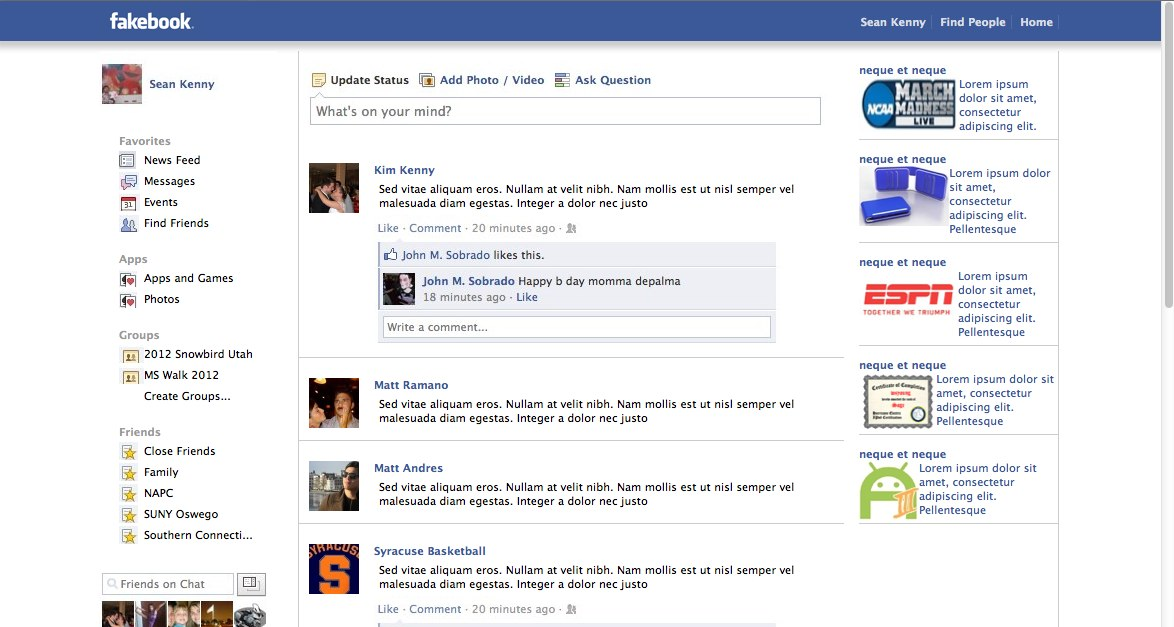
\includegraphics[width=\textwidth,keepaspectratio]{figures/images/sample_app.jpg}
\caption{Feature rich OpenPipe sample application to illustrate nested pipelines}
\end{figure}

The static application contains a diverse amount of sections. The resulting HTML, CSS, and JavaScript code created during this page creation was migrated to an MVC Based system that implements the OpenPipe Adapter interface.


\section{Basic Pipeline}

During the initial prototyping phase for OpenPipe a basic pipelined base site was built to illustrate the core components that are applied during the main pipeline process.The basic pipeline example is composed of one default layout, and three separate page pipelets [see figure \ref{fig:basicPipeline}]. 

\begin{figure}[H]
\label{fig:basicPipeline}
\centering
\fbox{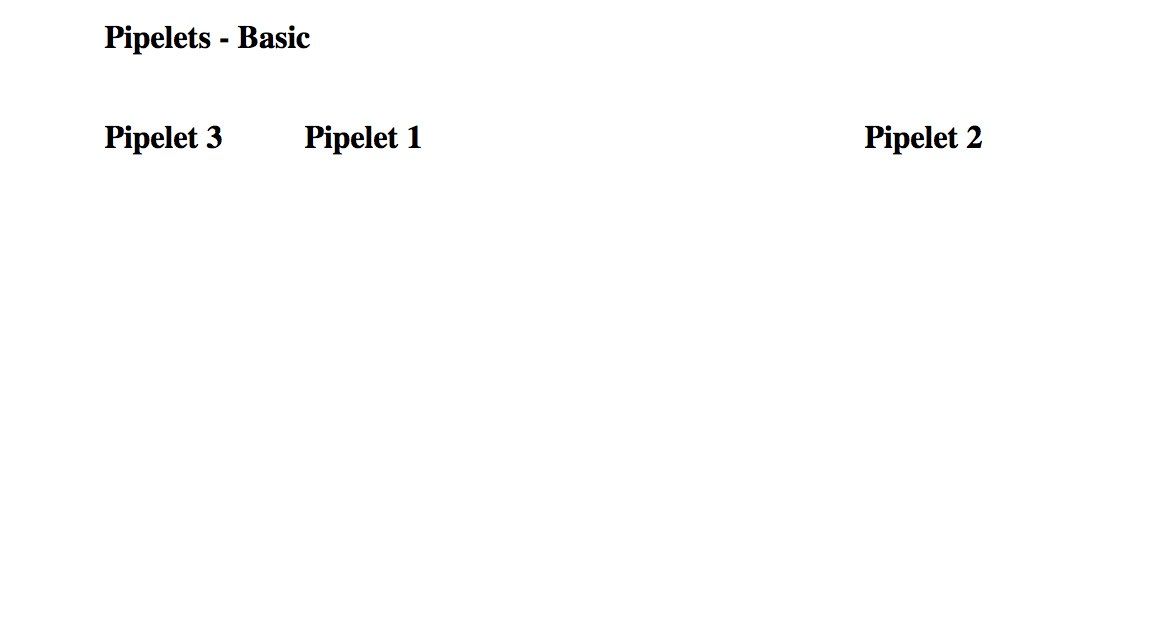
\includegraphics[width=\textwidth,keepaspectratio]{figures/images/basic_pipeline.jpg}}
\caption{Basic OpenPipe sample application to illustrate a basic pipelines}
\end{figure}

This simple design did not integrate with any existing PHP frameworks and relied on a very simple paradigm available in the PHP language called includes. Each pipelet being loaded is placed in an include file within a defined folder specified at runtime. The root Pipelet layout is placed within the layout.php include file,	 which is also specified at runtime. This simple and effective OpenPipe application was used to verify and test all the components of the OpenPipe system including the client side JavaScript library. 


\section{MVC Pipeline (PVC)}

The final stage in the development cycle was to implement an adapter for an existing PHP MVC framework. This adapter essentially retrofits the existing framework, and allows it to take advantage of HTTP pipelining provided by the OpenPipe library. 

The PHP MVC framework chosen to create an adapter for is named CodeIgniter. CodeIgniter is a lightweight open-source MVC framework, that is relatively simple to work with and extend. 

Utilizing CodeIgniter’s same system of controllers and views, a developer can easily convert any CodeIgniter page to an HTTP pipelined request. This is made possible by a simples series of installation steps illustrated in the provided sample application. The main index file ends of looking like figure \ref{fig:codeIgniterPvcCode}, once the OpenPipe integration has taken place.

\begin{figure}[H]
\label{fig:codeIgniterPvcCode}
\begin{lstlisting}
<?php
require_once(dirname(__FILE__).'/../../../server/php/OpenPipe/Adapter/Pvc/CodeIgniter.php');
require_once(dirname(__FILE__).'/../../../server/php/OpenPipe/Output/Piped.php');
require_once(dirname(__FILE__).'/../../../server/php/OpenPipe/Output/Standard.php');
require_once(dirname(__FILE__).'/../../../server/php/OpenPipe/Runner.php');

$openPipeAdapter = new OpenPipe_Adapter_Pvc_CodeIgniter(dirname(__FILE__));

if(isset($_GET['nopipe'])){
$openPipeOutput = new OpenPipe_Output_Standard();	
}else{
$openPipeOutput = new OpenPipe_Output_Piped('../../../../client/js');	
}
\end{lstlisting}
\caption{OpenPipe adapter setup for CodeIgniter}
\end{figure}


\section{Data Collection}

To collect data from the test applications a simple but powerful script [see figure \ref{fig:seleniumScript}] was developed utilizing the Selenium framework to automate the systematic retrieval of performance timing data for loaded web pages. The web page selected for data collection was the OpenPipe enabled static sample app previously illustrated [see figure \ref{fig:sampleApp}].  Selenium was a perfect candidate for automated retrieval of data, because unlike other types of web request tools such as cURL or wget which just send and receive raw HTTP data, Selenium drives a physical web browser through the utilizing of underlying browser API systems. The means that data is loaded and processed exactly the same as when an end user accesses a given website. This includes web requests, web reponses,  loading and unloading of the DOM,  and JavaScript execution. JavaScript execution was a crucial component in determining the load time for a OpenPipe enabled web page, since all data is unpacked and loaded in the browser via JavaScript after it has been received from the server.

\begin{figure}[H]
\label{fig:seleniumScript}
\begin{lstlisting}
#------------------------------------------------------------
# Script for recording performance timing of a given web page
# @author Sean Kenny <skenny214@gmail.com>
#------------------------------------------------------------
require 'pp'
require 'rubygems'
require 'csv'
require 'selenium-webdriver'

#get arguments
url = ARGV[0];
cycles = ARGV[1] || '5'
output_file = ARGV[2] || 'output.csv'

#open client driver for firefox
browser = Selenium::WebDriver.for :firefox

#open csv for writing output data
CSV.open(output_file, "w") do |csv|
	#for the amount of times the user wanted, get the page, get the performance timing, and output to csv
	cycles.to_i.times do |i|	
		browser.get url
		browser_timing = browser.execute_script("return window.performance.timing"); 
		openpipe_timing = browser.execute_script("return typeof(op) !== 'undefined' ? op.performance.timing.segments : null");

		# calculate wait time in two ways - if not openpipe then just use reponse start
		if(openpipe_timing == nil)
			browser_timing['responseWaitTime'] = browser_timing['responseStart'] - browser_timing['requestStart']

		#if we have openpipe timing then the response wait time is for first piece of actual content (assumed to be pipelet of first priority)
		else		
			browser_timing['responseWaitTime'] = openpipe_timing[1] - browser_timing['requestStart']
		end

		browser_timing['totalLoadWaitTime'] = browser_timing['loadEventEnd'] - browser_timing['requestStart'] 
		
		sorted_timing_values = []
		browser_timing.keys.sort.each do |key| 
			sorted_timing_values << browser_timing[key]
		end
		
		csv << browser_timing.keys.sort if i==0
		csv << sorted_timing_values
	end
end

browser.quit
\end{lstlisting}
\caption{A selenium script that retrieves performance and timing data from websites}
\end{figure}

Utilizing Selenium to load a web page also allowed for controlled access to performance timing information recorded by web browsers during each web request. This performance timing information can be found in the DOM javascript element, ' window.performance.timing'.  The data strucutre for window.performance.timing can be seen in figure \ref{fig:performanceTimingData}. To make the meaning of the data found withing the window.performance.timing data strucutre more clear a visualition timeline that illustrates when the performance timing events occur can be see in figure \ref{fig:performanceTimingChart}.


\begin{figure}[H]
\label{fig:performanceTimingData}
\begin{lstlisting}
interface PerformanceTiming {
  readonly attribute unsigned long long navigationStart;
  readonly attribute unsigned long long unloadEventStart;
  readonly attribute unsigned long long unloadEventEnd;
  readonly attribute unsigned long long redirectStart;
  readonly attribute unsigned long long redirectEnd;
  readonly attribute unsigned long long fetchStart;
  readonly attribute unsigned long long domainLookupStart;
  readonly attribute unsigned long long domainLookupEnd;
  readonly attribute unsigned long long connectStart;
  readonly attribute unsigned long long connectEnd;
  readonly attribute unsigned long long secureConnectionStart;
  readonly attribute unsigned long long requestStart;
  readonly attribute unsigned long long responseStart;
  readonly attribute unsigned long long responseEnd;
  readonly attribute unsigned long long domLoading;
  readonly attribute unsigned long long domInteractive;
  readonly attribute unsigned long long domContentLoadedEventStart;
  readonly attribute unsigned long long domContentLoadedEventEnd;
  readonly attribute unsigned long long domComplete;
  readonly attribute unsigned long long loadEventStart;
  readonly attribute unsigned long long loadEventEnd;
};
\end{lstlisting}
\caption{DOM performance timing data made available via JavaScript \cite{w3cNavigationTiming}}
\end{figure}


\begin{figure}[H]
\caption{DOM performance timing data show as linear request \cite{w3cNavigationTiming}}
\label{fig:performanceTimingChart}
\centering
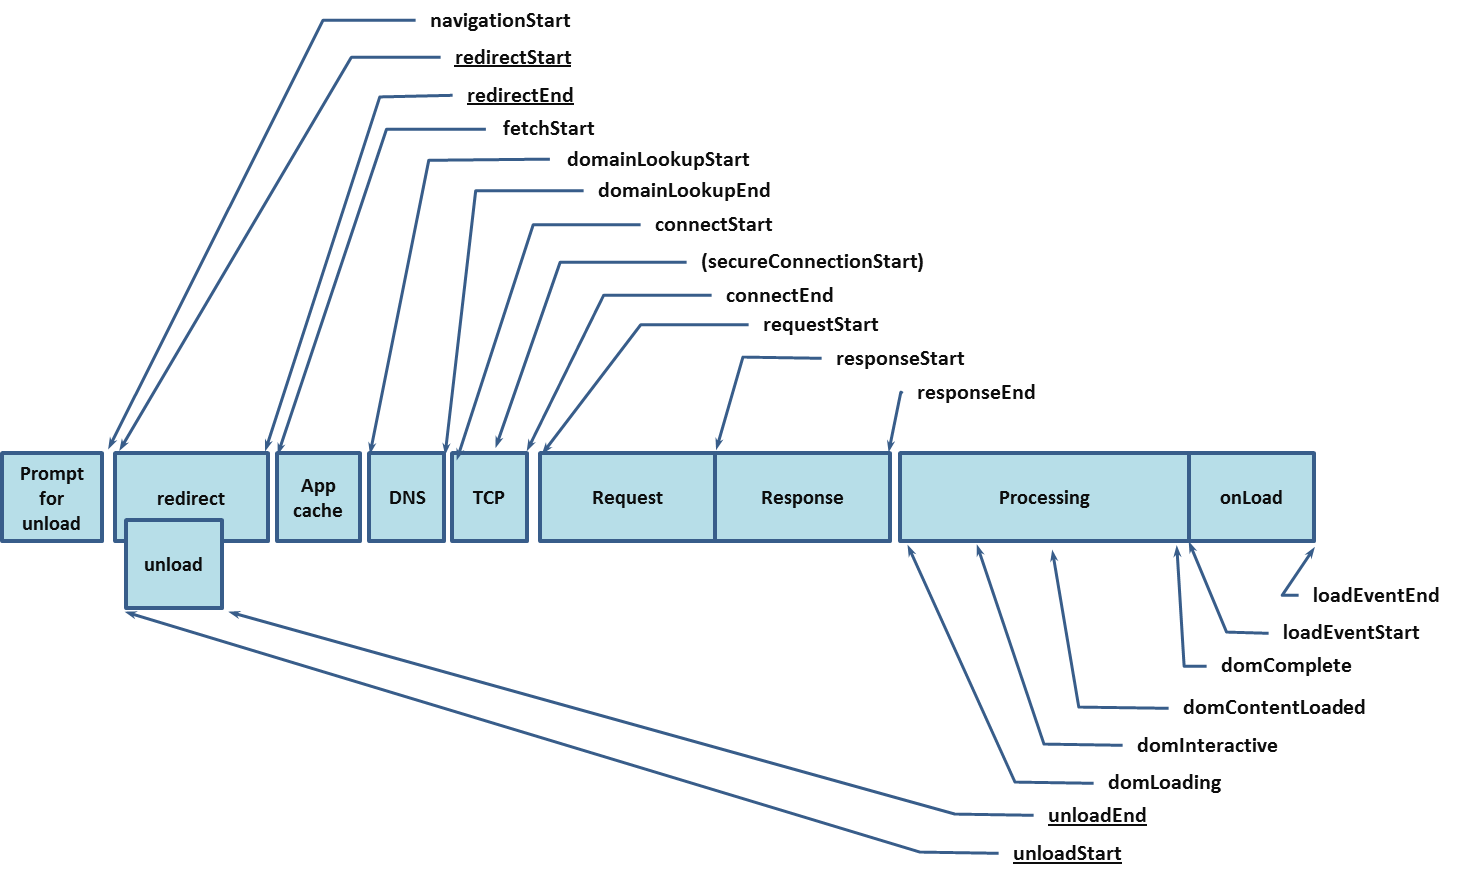
\includegraphics[width=150mm]{figures/images/timing_overview.png}
\end{figure}

\section{Simulating Load}

One important charactertistic to consider when developiong a web based library is how it performs unders load. The dimension of load that was considered when performance testing OpenPipe was the number of concurrent connections the server was able to process, and how this affected overall performance with and without the OpenPipe library outputting data through an HTTP data pipeline.

To achieve an accurate simulation of load the freely available and opensource tool named, 'Siege', was utilized. Siege is an HTTP web server load testing and benchmarking utility. It was designed to let web developers measure their code under stress, and see how it will stand up to load while in a production environment \cite{siegeHomepage}.  Siege allows for easily specificy the number of concurrent virtual users that should be tested accessing the site. The concurrency level is set using the -c flag when invoking the siege command line utility program. This concurrency option is descibed in the Siege manual in as the following:

\begin{quote}
This option allows the user to stress the web server with the number of simulated users. The amount is limited only by the computing resources available, but realistically a couple of hundred simulated users is equal to many times that that number in actual user sessions. The number you select represents the number of transactions your server is handling \cite{siegeManual}.
\end{quote}

 OpenPipe was tested while siege was run at concurrency levels 10, 25, 50, and 100. 
 

\chapter{RESULTS AND ANALYSIS}

\section{Performance Timing Table Data}
Once the performance timing data was collected additional data points were calculated to clarify if any performance benefits could be found between a pipelined and non-pipelined version a webpage. This data was collected and laid out in a tabular format [see figure \ref{fig:performanceTimingTable}]. The columns in the presented table represent the following variables and formulas:

\begin{enumerate}
\item \textbf{Type} - Represents the type of external event that the server is issuing to complete the given web page request. Three types of web page requests were simulated:
	\begin{enumerate}
	\item \textbf{Plain HTML} - The server does not connect to any external system. It simply renders and return HTML content. This HTML content also includes CSS and JavaScript.
	\item \textbf{Database} - The server creates a connection to a local database system and issues select queries over this connection to gather data. The data is not used in the display of the web page, but nevertheless this simulates the overhead necessary to connect to a local database system, loop through the data, and return a result.
	\item \textbf{Web Service} - The server create a connection to an external REST based web service. For the purposes of these tests the server connect to the twitter REST API and issues REST based query commands. The data is not used in the display of the web page, but nevertheless this simulates the overhead necessary to connect to an external REST based system, loop through the data, and return a result.
	\end{enumerate}
\item \textbf{Load} - The ammount of load that is being put on the web server during the testing time. Load was simulated using the command line tool named, 'Siege'. The number presented in this column represents the total number of concurrent connection being issued from Siege during the tests.
\item \textbf{Response} - The initial response time for a non piped page. The formula for this data point is: \begin{math} responseStart - requestStart \end{math} 
\item \textbf{Response Piped} - The initial response time for a non piped page. This is calculated by recording the load time of the first piece of content within a pipelet (users sees something) and comparing that to the request start time. The formula for this data point is: \begin{math} firstPipeletLoadTimeEnd - requestStart \end{math} 
\item \textbf{Total Time} and \textbf{Total Time Piped}   - The total time it took to the load the page, starting at request start and ending at the final DOM loaded event. The formula for this data point is: \begin{math} loadEventEnd - requestStart \end{math} 
\end{enumerate}


\begin{figure}[H]
\label{fig:performanceTimingTable}
\small
\begin{tabular}{llllll}
\textbf{Type}			&\textbf{Load}		&\textbf{Response}	&\textbf{Response Piped}	&\textbf{Total Time}	&\textbf{Total Time Piped}  	\\
\hline
\hline
\emph{Plain HTML}		& 0				& 80.81632653	& 56.10204082 (69\%)		& 102.6122449		& 144.0408163			\\
\emph{Database}		& 0				& 149.0612245	& 74.14285714 (50\%)		& 166.5714286		& 127.6122449			\\
\emph{Web Service}		& 0				& 5144.959184	& 795.2244898 (15\%)		& 5164.77551			& 5103.959184			\\
\hline
\emph{Plain HTML}	  	& 10				& 141.9183673	& 90.51020408 (64\%)		& 187.4489796		& 172.3469388    			\\
\emph{Database}		& 10 			& 408.8367347	& 231.8979592 (57\%)		& 448.4081633		& 618.7142857  			\\
\emph{Web Service}		& 10				& 5053.040816	& 767.5510204 (15\%)		& 5110.591837		& 5114.691837    			\\
\hline
\emph{Plain HTML}		& 25				& 137.1836735	& 85.02040816 (62\%)		& 184.4285714		& 192.8163265    			\\
\emph{Database}		& 25				& 2583.612245	& 939.6530612 (36\%)		& 2621.387755		& 2649.897959    			\\
\emph{Web Service}		& 25				& 4872.367347	& 718.8775510 (15\%)		& 4912.204082		& 5177.857143   			 \\
\hline
\emph{Plain HTML}		& 50				& 146.9591837	& 111.5306122 (76\%)		& 194				& 220.8979592   			\\
\emph{Database}		& 50				& 6172.265306	& 2203.897959 (36\%)		& 6214.673469		& 6244.55102    			\\
\emph{Web Service}		& 50				& 4791.755102	& 750.2857143 (16\%)		& 4848.040816		& 4790.081633    			\\
\hline
\emph{Plain HTML}		& 100			& 149.2653061	& 102.7959184 (69\%)		& 192.8979592		& 195.3673469    			\\
\emph{Database}		& 100			& 12139.69388	& 4530.346939 (37\%)		& 12217.28571		& 12878.77551    			\\
\emph{Web Service}		& 100			& 4742.285714	& 741.6734694 (16\%)		& 4827.040816		& 4754.469388    			\\
\end{tabular}
\caption{Calculated response and load time in milliseconds. Data is based on timing data collected from automated browser runs via Selenium scripting.}
\end{figure}


\section{Charts}
Utilizing the data collected in figure \ref{fig:performanceTimingTable} a bar chart was created for each external service type, and  each service type was compared with changes in load to the server.  The charts can be seen in figures 11.1, 11.2, and 11.3.

\begin{figure}[H]
\label{fig:analysisChartPlain}
\centering
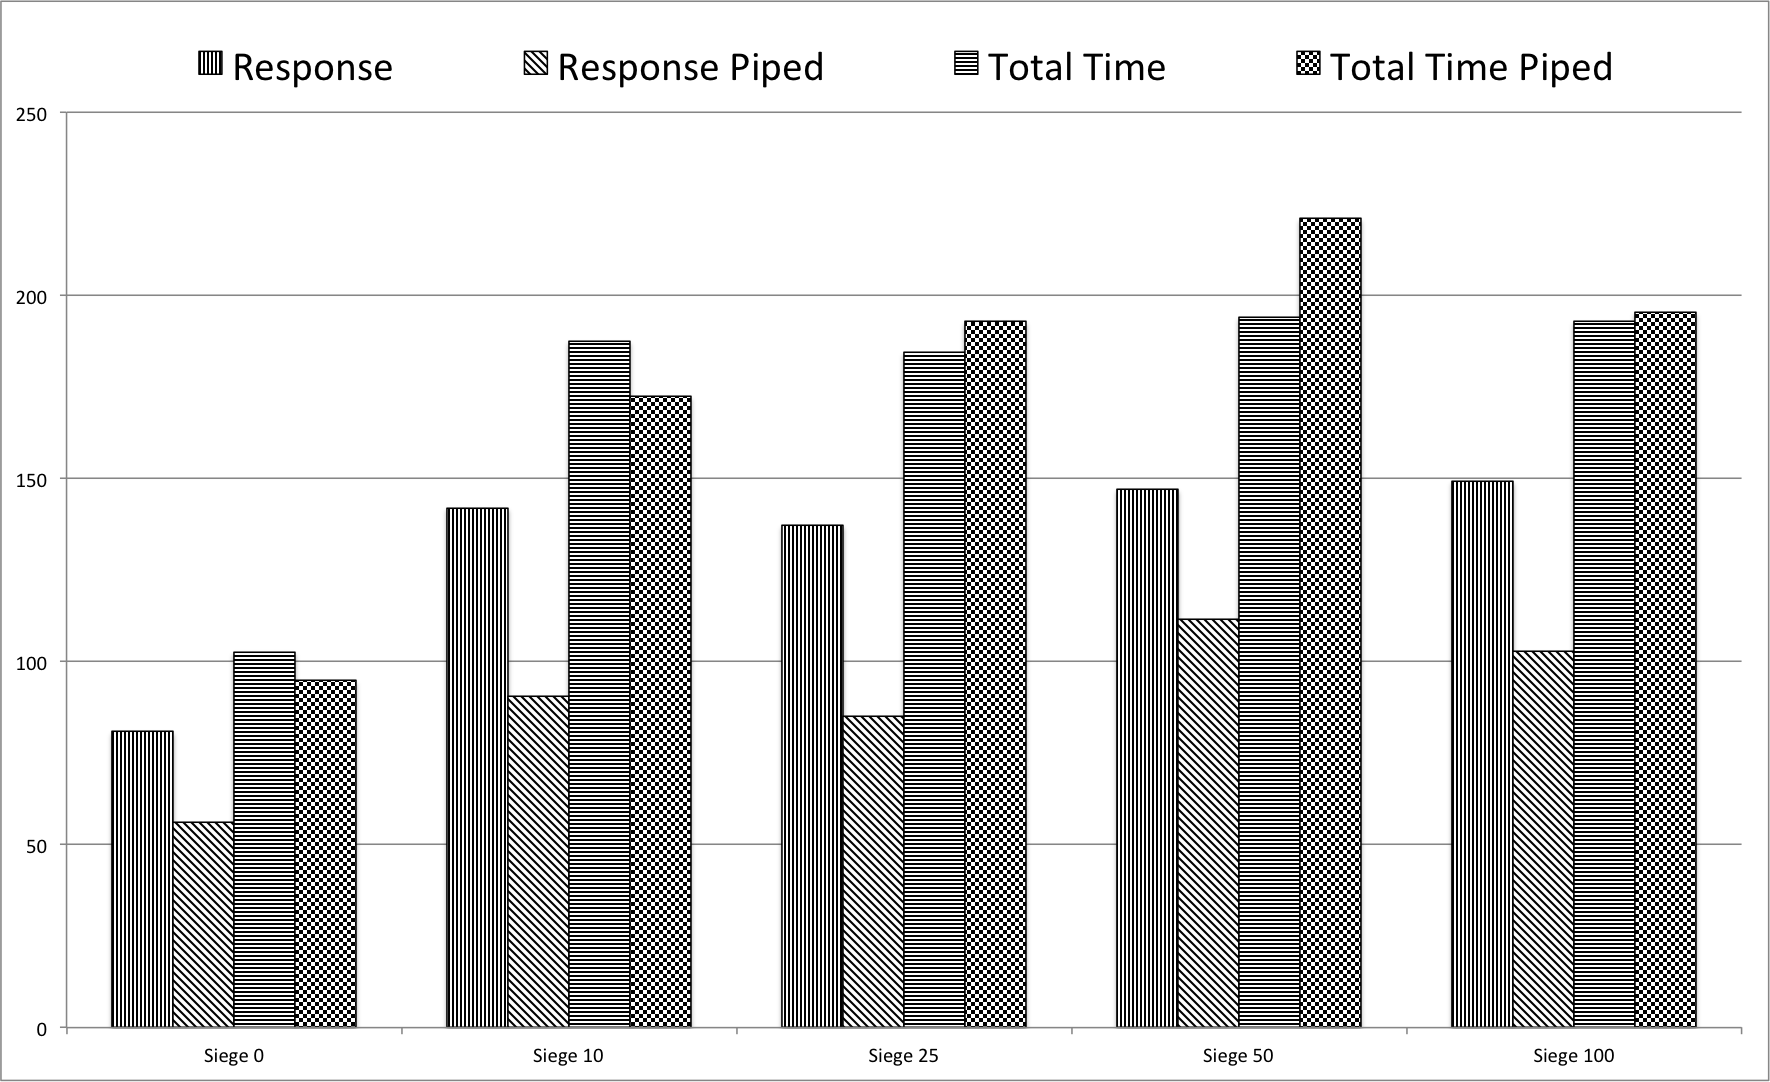
\includegraphics[width=\textwidth,keepaspectratio]{figures/images/analysis_chart_plain.png}
\caption{OpenPipe column chart comparing non-piped vs. piped response times and total load times for plain HTML data}
\end{figure}

\begin{figure}[H]
\label{fig:analysisChartDatabase}
\centering
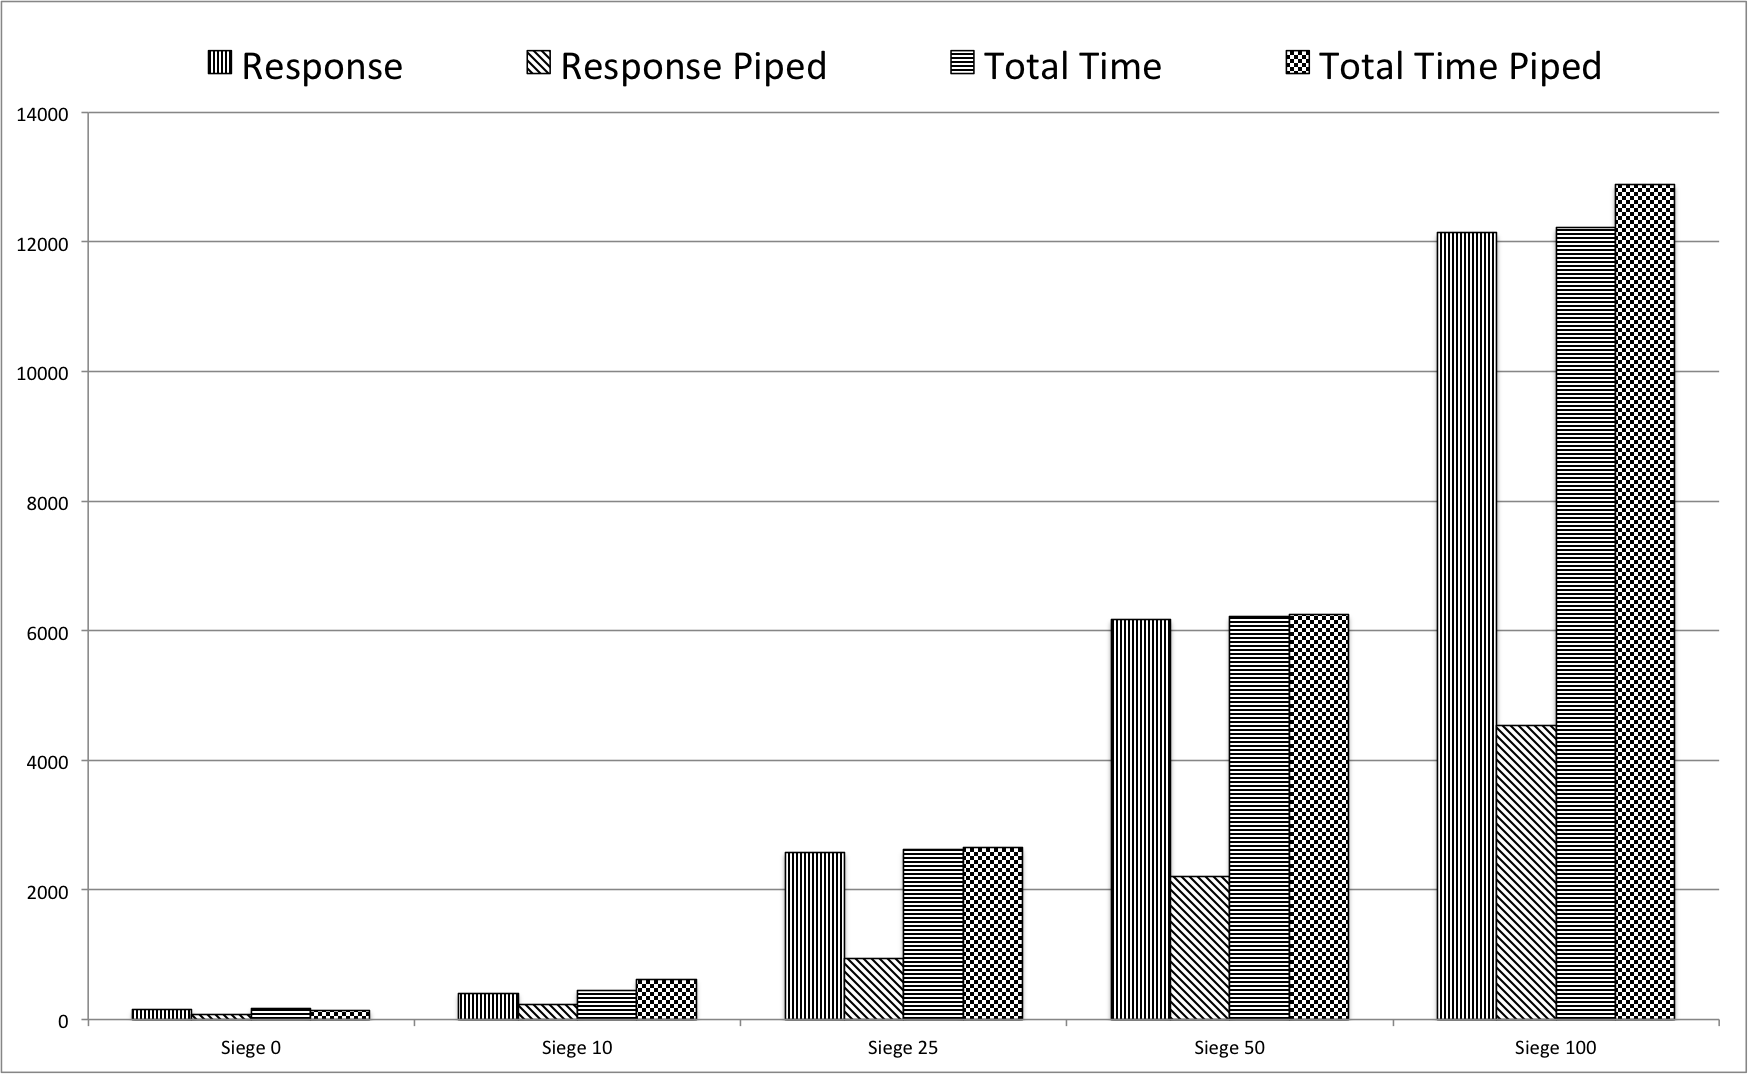
\includegraphics[width=\textwidth,keepaspectratio]{figures/images/analysis_chart_database.png}
\caption{OpenPipe column chart comparing non-piped vs. piped response times and total load times when connecting to a local database system for data}
\end{figure}

\begin{figure}[H]
\label{fig:analysisChartWebService}
\centering
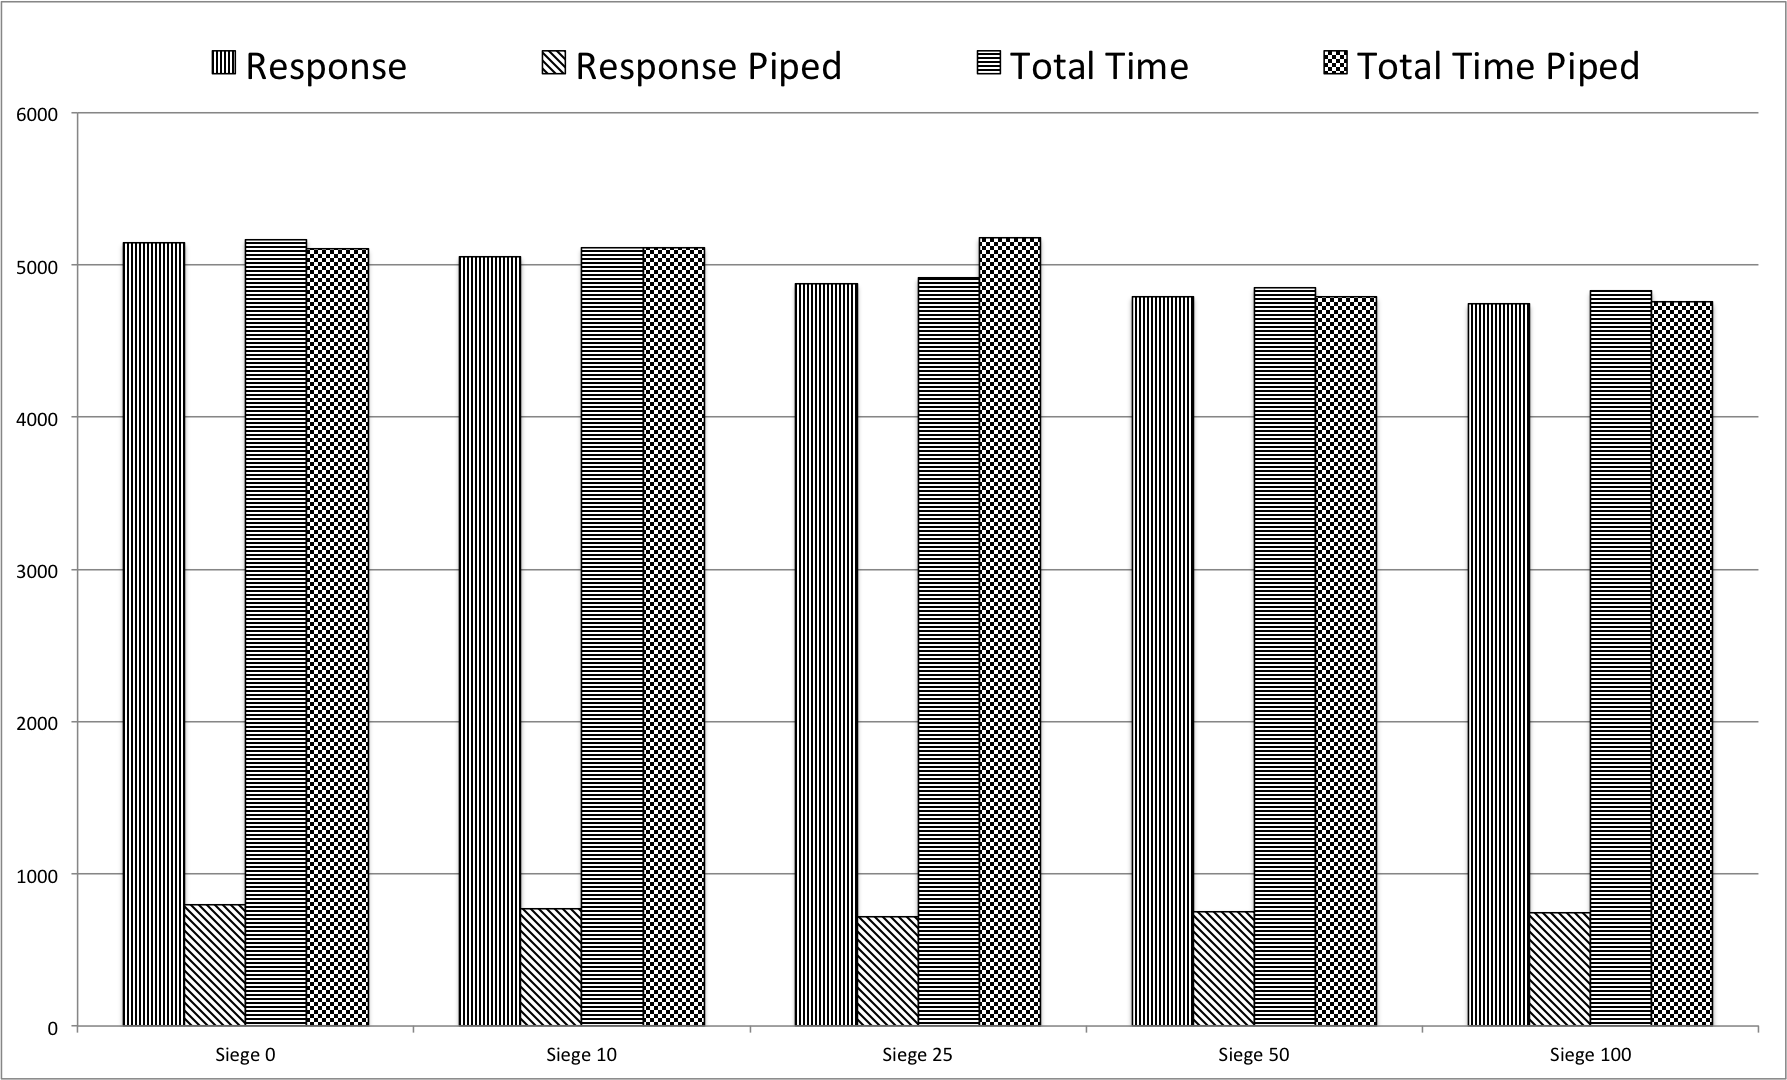
\includegraphics[width=\textwidth,keepaspectratio]{figures/images/analysis_chart_webservice.png}
\caption{OpenPipe column chart comparing non-piped vs. piped response times and total load times when connecting to an external REST API for data}
\end{figure}

\section{Conclusions}
The following items can be extracted from the presented table data and charts:

\begin{enumerate}
\item On average across all type of requests and server load a piped request requires only 38\% of the time that would be needed to send a non-piped version of the same page.
\item Requests that involve calls to external web services see the biggest performance gains. This is due to the overhead required for a server to send and receive requests from an external web service running on another server. If many requests to an external service must be made for a single page, then a piped version of the same page will gain a significent performance advantage over the non-piped counterpart.
\item Piped versions of pages do. on average, require more time to load. Although the increased time is usually insignificent when compared to the speed gained in initial response time. Total page load time increasing is to be expected due to the additional overhead in client side processing to unpack and load the page pipelets when they arrive from the server. 
\item Overall load on the server caused the greatest increase in response time when sending database type requests. This is due to the increased load on a single server environment caused by simultaneious connections to the local web server and local database server. 
\end{enumerate}

In general the results are very promising.  They illustrate how an an HTTP pipeline like OpenPipe can result in large benefits in terms of of response time for a given web page that requires access to one to many external systems for data or storage. This decreased initial response time can speed up the perceived load time of the web page. In general there seems to be very little negeative tradeoffs when incorporating OpenPipe into a web based system.

%------------------------------------------------------------------------------------------------------
%--------------------Discussion-------------------------------------------------------------------------
%------------------------------------------------------------------------------------------------------
\chapter{FUTURE WORK}

\section{Expanded Output API}

Right now the OpenPipe system relies an an implicit layout output system that is integrated into a new or existing web framework. The API could be extended to provide a more explicit type of output system that may be useful in some scenarios that a developer may encounter. An example of an explicit API that could  be developed can be found in figure \ref{fig:explicitApi}

\begin{figure}[H]
\label{fig:explicitApi}
\begin{lstlisting}
<?php
$layoutData = file_get_contents('layout.php');

$pipe = new OpenPipe_Output_Handle();
$pipe->sendLayout($layoutData);

$dbRecords = mysql_query('select * from facts');
$content = '';
foreach($dbRecords as $dbRecord){
	$content .= "<h1>User {$dbRecord['user_name']}</h1>";
}

$pipe->sendContent('user-names', $content);
$pipe->endPhase(1);
$pipe->close();
?>
\end{lstlisting}
\caption{An explicit version of an OpenPipe output API}
\end{figure}

\section{Minification}
The OpenPipe output adapter could add another output step where JavaScript, CSS, and HTML code is minified. Minified code has all unnecessary characters removed from its content, without changing the functionality of the original program. Minification can play an important role in further optimizing the pipeline by reducing the overall size of individual pipelet components.

\section{Addition of framework adapters}
Out of the box OpenPipe allows for integration with the CodeIgniter MVC Framework. Utilizing the strategy design pattern it is possible to developer additional adapters that allow for integration with existing and future PHP frameworks. Some frameworks that would be next to integrate include:

\begin{enumerate}
	\item Symfony
	\item Zend Framework
	\item CakePHP
	\item Yii
\end{enumerate}

\section{Language agnostic Apache server extension}
Currently the OpenPipe library is limited to working with PHP based applications and websites. This is due to the fact that the entire server side implementation is built  using the PHP language and is executed by the web server using additional modules like mod\_php. 

Web servers like apache provide application interfaces for developing server extensions. OpenPipe development could progress to include an embedded apache module that allows for integration with any web based applications utilizing any web scripting language. This would allow OpenPipe to integrate with tools such as Python, Ruby, and Perl.




%------------------------------------------------------------------------------------------------------
%--------------------CODE LISTINGS ---------------------------------------------------------------------
%------------------------------------------------------------------------------------------------------
\appendix
\singlespacing
\addtocontents{toc}{\def\protect\cftchappresnum{APPENDIX }}

\chapter{SERVER SOURCE CODE}
%--------- SERVER PHP FILES ---------- 
\section{Pipelet/Runner.php}
\phplist{OpenPipe/Runner.php}

\section{Pipelet/Interface.php}
\phplist{OpenPipe/Pipelet/Interface.php}

\section{Pipelet/Abstract.php}  
\phplist{OpenPipe/Pipelet/Abstract.php}

\section{Pipelet/Base.php} 
\phplist{OpenPipe/Pipelet/Base.php}

\section{Pipelet/Factory.php} 
\phplist{OpenPipe/Pipelet/Factory.php}

\section{Output/Interface.php} 
\phplist{OpenPipe/Output/Interface.php}

\section{Output/Piped.php} 
\phplist{OpenPipe/Output/Piped.php}

\section{Output/Standard.php} 
\phplist{OpenPipe/Output/Standard.php}

\section{Output/Util.php} 
\phplist{OpenPipe/Output/Util.php}

\section{Adapter/Interface.php} 
\phplist{OpenPipe/Adapter/Interface.php}

\section{Adapter/Abstract.php} 
\phplist{OpenPipe/Adapter/Abstract.php}

\section{Adapter/Basic.php} 
\phplist{OpenPipe/Adapter/Basic.php}

\section{Pvc/CodeIgniter.php} 
\phplist{OpenPipe/Adapter/Pvc/CodeIgniter.php}

%--------- CLIENT JS FILES---------- 
\chapter{CLIENT SOURCE CODE}

\section{openpipe.js} 
\jslist{openpipe.js}



%------------------------------------------------------------------------------------------------------
%--------------------BIBLIOGRAPHY ---------------------------------------------------------------------
%------------------------------------------------------------------------------------------------------
\begin{thebibliography}{2}
\doublespacing

\bibitem{facebookBigpipe}
facebook.com, "BigPipe: Pipelining web pages for high performance", Facebook, June 2010 [Online]
Available: http://www.facebook.com/notes/facebook-engineering/bigpipe-pipelining-web-pages-for-high-performance/389414033919 [Retrieved December 2010]

\bibitem{hypertextTransferProtocol}
w3.org, "Part of Hypertext Transfer Protocol -- HTTP/1.1 – 8 - Connections", W3C/MIT, June 1999 [Online]
Available: http://www.w3.org/Protocols/rfc2616/rfc2616-sec8.html [Retrieved December 2010]

\bibitem{optimizingPageLoadTime}
Aaron Hopkins, "Optimizing Page Load Time", die.net [Online]
Available: http://www.die.net/musings/page\_load\_time/ [Retrieved December 2010]

\bibitem{whatIsPipelining}
Darin Fisher, "What is HTTP pipelining", Mozilla, April 2008 [Online]
Available: http://www.mozilla.org/projects/netlib/http/pipelining-faq.html [Retrieved December 2010]

\bibitem{w3cNavigationTiming}
Zhiheng Wang, "Navigation Timing", W3C, July 2012 [Online]
Available: dvcs.w3.org/hg/webperf/raw-file/tip/specs/NavigationTiming/Overview.html [Retrieved November 2012]

\bibitem{siegeHomepage}
Jeff Fulmer, "Siege Home",  joedog.org, January 2012 [Online]
Available: www.joedog.org/siege-home [Retrieved November 2012]

\bibitem{siegeManual}
Jeff Fulmer, "Siege Manual", joedog.org, January 2012 [Online]
Available: http://www.joedog.org/siege-manual/ [Retrieved November 2012]

\bibitem{phpWiki}
wikipedia.org, "PHP", Wikimedia Foundation [Online]
Available: http://en.wikipedia.org/wiki/PHP [Retrieved October 2012]

\bibitem{webserverSurvey}
netcraft.com, "March 2012 Web Server Survey", Netcraft [Online]
Available: http://news.netcraft.com/archives/2012/03/05/march-2012-web-server-survey.html [Retrieved October 2012]

\bibitem{highPerformanceWebsites}
Steve Souders, High Performance Websites, Oreilly Media, September 2007

\bibitem{evenFasterWebsites}
Steve Souders, Even Faster Web Sites: Performance Best Practices for Web Developers, Oreilly Media, June 2009

\end{thebibliography}

\end{document}
